% !TeX root = ..\main.tex
\section{Lược đồ Use-case}
\subsection{Toàn hệ thống}
\begin{figure}[!htp]
    \centering    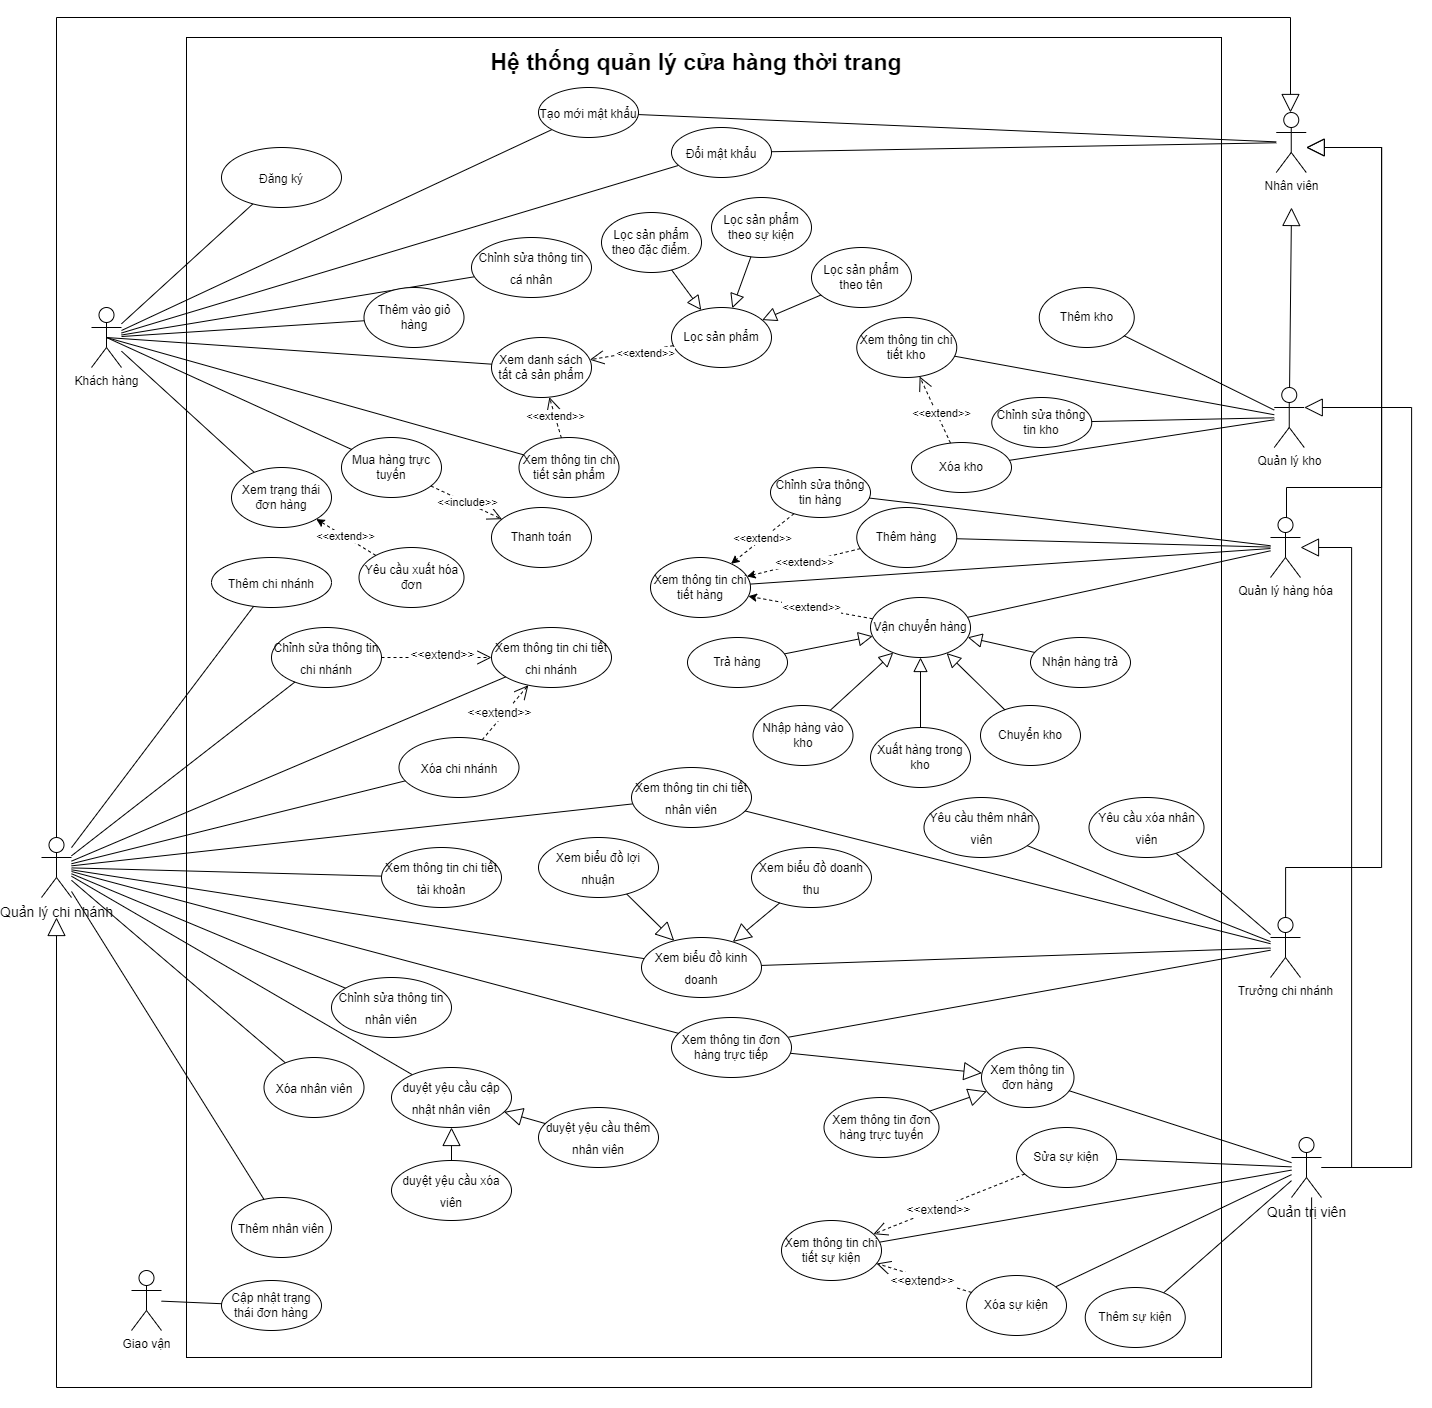
\includegraphics[width=16.5cm]{img/UseCase/UseCase-full.drawio.png}
    \newline
    \caption{Use case Hệ thống quản lý cửa hàng thời trang}
\end{figure}
\textbf{Lưu ý:} Các Usecase không yêu cầu đăng nhập:
\begin{itemize}
\item Đăng ký
\item Tạo mới mật khẩu
\item Xem danh sách sản phẩm
\item Lọc sản phẩm
\item Điểm danh
\end{itemize}
\newpage


\subsection{Đặt hàng trực tuyến}

     \begin{figure}[!htp]
        \centering
        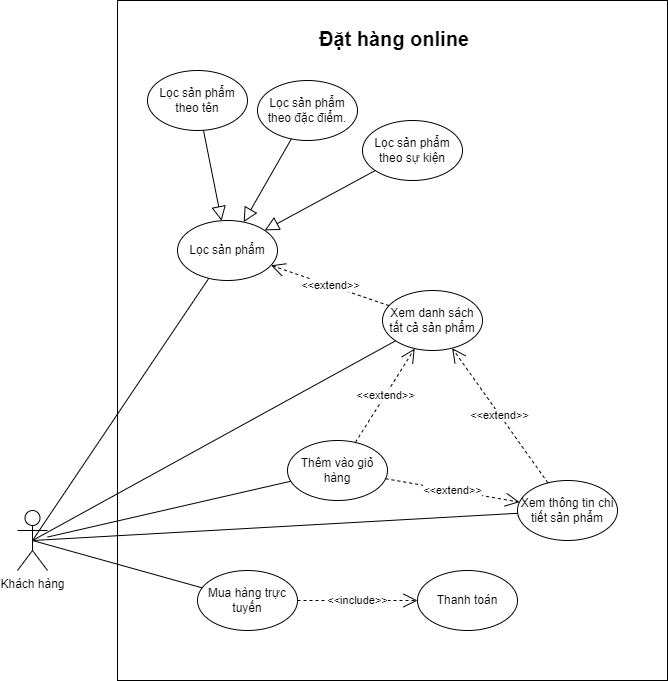
\includegraphics[width=12cm]{img/UseCase/UseCase-Đặt hàng.drawio.png}
        \newline
        \caption{Use case đặt hàng trực tuyến}
    \end{figure}
    \subsubsection{Xem danh sách sản phẩm} 
            \begin{center}
            
                \begin{longtable}{| p{.20\textwidth} | p{.80\textwidth} |} 
    \hline
    \textbf{Use-case name}
    & 
    Xem danh sách sản phẩm
    \\
    \hline
    \textbf{Actor} 
    & 
    Người dùng
    \\
    \hline
    \textbf{Description} 
    & 
    Cho phép người dùng có thể xem danh sách các sản phẩm của cửa hàng.
    \\
    \hline
     \textbf{Preconditions} 
    &
    Người dùng đã truy cập vào trang chủ của nhà hàng.
    \\
    \hline
    \textbf{Postconditions} 
    & 
    Người dùng xem được danh sách các sản phẩm thời trang của cừa hàng.
    \\
    \hline
    \textbf{Trigger} 
    & 
    Không.
    \\
    \hline
     \textbf{Normal flow}
    & 
        1. Hệ thống hiển thị các sản phẩm theo mặc định.
        
        2. Người dùng chọn mục tất cả sản phẩm.
        
        3. Hệ thống hiển thị toàn bộ sản phẩm có bán trong cửa hàng.
        
        4. Người dùng lướt trang web để duyệt tất cả các sản phẩm của cửa hàng.
    \\
    \hline
    \textbf{Alternative flow}
    & 
        2.1 Người dùng lướt trang chủ để xem các sản phẩm nổi bật mặc định của trang web.
    \\
    %%%%%%%%%%%%%%%%
    \hline
    \textbf{Exceptions} 
    &
    Không
    %%%%%%%%%%%%%%%%%%%%
    \\
    \hline
    \caption{Đặc tả use-case \textbf{xem danh sách sản phẩm}}
    \end{longtable}
                    
            \end{center}


    \subsubsection{Lọc sản phẩm theo từ khóa} 
            \begin{center}
            
                \begin{longtable}{| p{.20\textwidth} | p{.80\textwidth} |} 
    \hline
    \textbf{Use-case name}
    & 
    Lọc danh sách sản phẩm theo từ khóa
    \\
    \hline
    \textbf{Actor} 
    & 
    Người dùng
    \\
    \hline
    \textbf{Description} 
    & 
    Cho phép người dùng có thể xem danh sách các sản phẩm của cửa hàng có chứa tên mà người dùng mong muốn.
    \\
    \hline
     \textbf{Preconditions} 
    &
    Người dùng đã truy cập vào trang chủ của nhà hàng.
    \\
    \hline
    \textbf{Postconditions} 
    & 
    Người dùng xem được danh sách các sản phẩm  của cừa hàng có tên chứa từ khóa mà người dùng muốn xem.
    \\
    \hline
    \textbf{Trigger} 
    & 
    Không.
    \\
    \hline
     \textbf{Normal flow}
    & 
        1. Hệ thống hiển thị các sản phẩm theo mặc định.
        
        2. Người dùng nhập từ khóa của sản phẩm muốn tìm.
        
        3. Hệ thống hiển thị toàn bộ sản phẩm mà tên có từ khóa mà khách hàng tìm kiếm.
        
        4. Người dùng xem kết quả danh sách sản phẩm tìm kiếm của hệ thống.
    \\
    \hline
    \textbf{Alternative flow}
    & 
    Không
    %%%%%%%%%%%%%%%%
    \\
    \hline
    \textbf{Exceptions} 
    &
    Không
    %%%%%%%%%%%%%%%%%%%%
    \\
    \hline
    \caption{Đặc tả use-case \textbf{lọc sản phẩm theo từ khóa}}
    \end{longtable}
    \end{center}
    

    \subsubsection{Lọc sản phẩm theo sự kiện }
            \begin{center}
            
                \begin{longtable}{| p{.20\textwidth} | p{.80\textwidth} |} 
    \hline
    \textbf{Use-case name}
    & 
    Lọc danh sách sản phẩm theo sự kiện
    \\
    \hline
    \textbf{Actor} 
    & 
    Người dùng
    \\
    \hline
    \textbf{Description} 
    & 
    Cho phép người dùng có thể xem các sản phẩm của cửa hàng đang trong danh sách thuộc sự kiện mà người dùng muốn xem.
    \\
    \hline
     \textbf{Preconditions} 
    &
    Người dùng đã truy cập vào trang chủ của nhà hàng.
    \\
    \hline
    \textbf{Postconditions} 
    & 
    Người dùng xem được các sản phẩm của cửa hàng đang trong danh sách thuộc sự kiện mà người dùng muốn xem.
    \\
    \hline
    \textbf{Trigger} 
    & 
    Không
    \\
    \hline
     \textbf{Normal flow}
    & 
        1. Hệ thống hiển thị các sự kiện trong trang mặc định
        .
        2. Người dùng chọn sự kiện muốn xem.
        
        3. Hệ thống hiển thị toàn bộ sản phẩm mà có trong danh sách thuộc sự kiện người dùng chọn.
        
        4. Người dùng xem kết quả danh sách sản phẩm sau khi lọc.
    \\
    \hline
    \textbf{Alternative flow}
    & 
    Không
    %%%%%%%%%%%%%%%%
    \\
    \hline
    \textbf{Exceptions} 
    &
    Không
    %%%%%%%%%%%%%%%%%%%%
    \\
    \hline
    \caption{Đặc tả use-case \textbf{lọc sản phẩm theo sự kiện}}
    \end{longtable}
                    
            \end{center}


    \subsubsection{Lọc sản phẩm theo đặc điểm } 
            \begin{center}
            
                \begin{longtable}{| p{.20\textwidth} | p{.80\textwidth} |} 
    \hline
    \textbf{Use-case name}
    & 
    Lọc danh sách sản phẩm theo đặc điểm
    \\
    \hline
    \textbf{Actor} 
    & 
    Người dùng
    \\
    \hline
    \textbf{Description} 
    & 
    Cho phép người dùng có thể xem các sản phẩm của cửa hàng có các đặc điểm của các thể loại mà người dùng chọn.
    \\
    \hline
     \textbf{Preconditions} 
    &
    Người dùng đã vào trang tất cả sản phẩm của nhà hàng.
    \\
    \hline
    \textbf{Postconditions} 
    & 
    Người dùng xem được các sản phẩm của cửa hàng có các đặc điểm của thể loại mà người dùng muốn xem.
    \\
    \hline
    \textbf{Trigger} 
    & 
    Người dùng chọn "Tất cả sản phẩm".
    \\
    \hline
    \begin{flushleft}
     \textbf{Normal flow}
    \end{flushleft}
    & 
        1. Người dùng chọn đặc điểm của các trường muốn lọc (Các trường này theo bao gồm giá, thương hiệu, gender, size, màu sắc, nhóm sản phẩm).
        
        2. Hệ thống hiển thị toàn bộ sản phẩm mà có các đặc điểm mà người dùng chọn.
        
        3. Người dùng xem kết quả danh sách sản phẩm sau khi lọc.
    \\
    \hline
    \textbf{Alternative flow}
    & 
    Không
    %%%%%%%%%%%%%%%%
    \\
    \hline
    \textbf{Exceptions} 
    &
    Không
    %%%%%%%%%%%%%%%%%%%%
    \\
    \hline
    \caption{Đặc tả use-case \textbf{lọc sản phẩm theo đặc điểm}}
    \end{longtable}
                    
            \end{center}
    
    
            \subsubsection{Xem thông tin chi tiết sản phẩm } 
         \begin{longtable}{| p{.20\textwidth} | p{.80\textwidth} |} 
    \hline
    \textbf{Use-case name} 
    & 
    Xem thông tin chi tiết sản phẩm
    \\
    \hline
    \textbf{Actor} 
    & 
    Người dùng
    \\
    \hline
    \textbf{Description} 
    & 
    Cho phép người dùng có thể xem thông tin chi tiết của sản phẩm.
    \\
    \hline
    \textbf{Preconditions} 
    &
    Người dùng đang xem danh sách các sản phẩm.
    \\
    \hline
    \textbf{Postconditions} 
    & 
    Người dùng xem được thông tin chi tiết của sản phẩm mà người dùng muốn xem.
    \\
    \hline
    \begin{flushleft}
    \textbf{Normal flow}
    \end{flushleft}
    & 
        1. Người dùng chọn vào sản phẩm muốn xem trong danh sách các sản phẩm đang xem.
        
        2. Hệ thống hiển thị thông tin chi tiết của sản phẩm
        .
        3. Người dùng xem thông tin chi tiết của sản phẩm.
    \\
    \hline
    \textbf{Alternative flow}
    & 
    1.1. Người dùng xem danh sách sản phẩm trong giỏ hàng.
    
    1.2. Người dùng xem danh sách sản phẩm trong lịch sử mua hàng.
    %%%%%%%%%%%%%%%%
    \\
    \hline
    \textbf{Exceptions} 
    &
    Không
    %%%%%%%%%%%%%%%%%%%%
    \\
    \hline
    \caption{Đặc tả use-case \textbf{xem thông tin chi tiết sản phẩm}}
    \end{longtable}


    \subsubsection{ Thêm sản phẩm vào giỏ hàng}    
            
            \begin{longtable}{| p{.20\textwidth} | p{.80\textwidth} |} 
    \hline
    \textbf{Use-case name} 
    & 
    Thêm sản phẩm vào giỏ hàng
    \\
    \hline
    \textbf{Actor} 
    & 
    Người dùng
    \\
    \hline
    \textbf{Description} 
    & 
    Cho phép người dùng thêm sản phẩm vào giỏ hàng của tài khoản của họ.
    \\
    \hline
    \textbf{Preconditions} 
    &
    Người dùng đã đăng nhập vào hệ thống.
    \\
    \hline
    \textbf{Postconditions} 
    & 
    Người dùng thêm sản phẩm vào giỏ hàng của tài khoản của họ.
    \\
    \hline
    \textbf{Triggers} 
    &
    Không.
    \\
    \hline
    \begin{flushleft}
    \textbf{Normal flow}
    \end{flushleft}
    & 
        1. Người dùng chọn vào xem danh sách các sản phẩm.
        
        2. Hệ thống hiển thị danh sách các sản phẩm của người dùng chọn
        
        3. Người dùng chọn xem thông tin chi tiết sản phẩm.
        
        4. Hệ thống hiển thị thông tin chi tiết sản phẩm.
        
        5. Người dùng chọn các thông tin sản phẩm theo ý muốn (Thông tin bao gồm size, màu... tùy thuộc loại sản phẩm).
        
        6. Hệ thống thực hiện yêu cầu và hiển thị kết quả.
        
        7. Người dùng nhận kết quả thêm vào giỏ hàng thành công.
    \\
    \hline
    \begin{flushleft}
    \textbf{Alternative flow}
    \end{flushleft}
    & 
        1.1 Người dùng thêm vào giỏ từ lịch sử mua hàng.
        \begin{quote}
            1.1.1. Người dùng chọn xem đơn hàng đã mua.

            1.1.2. Hệ thống hiển thị danh sách các đơn hàng đã mua của người dùng.
        
            1.1.3. Người dùng chọn thêm lại vào giỏ hàng.
            
            1.1.4. Hệ thống thực hiện yêu cầu và hiển thị kết quả.
            
            1.1.5. Người dùng nhận kết quả thêm vào giỏ hàng thành công.
        
        \end{quote}
        3.1 Người dùng chọn thêm nhanh vào giỏ hàng.
        \begin{quote}
            3.1.1 Hệ thống thêm sản phẩm vào giỏ hàng của khách hàng với các thông tin mặc định của hệ thống và thông báo kết quả.
            
            3.1.2. Đến bước 7.
        \end{quote} 
    %%%%%%%%%%%%%%%%
    \\
    \hline
    \begin{flushleft}
        \textbf{Exceptions} 
    \end{flushleft}
    &
    7.1.Thêm vào giỏ hàng thất bại.
        \begin{quote}
            7.1.1 Quay lại bước 5.
        \end{quote}
    %%%%%%%%%%%%%%%%%%%%
    \\
    \hline
    \caption{Đặc tả use-case \textbf{thêm sản phẩm vào giỏ hàng}}
    \end{longtable}


    \subsubsection{Mua hàng trực tuyến }                 
        \begin{longtable}{| p{.20\textwidth} | p{.80\textwidth} |} 
    \hline
    \textbf{Use-case name} 
    & 
    Mua hàng trực tuyến
    \\
    \hline
    \textbf{Actor} 
    & 
    Người dùng
    \\
    \hline
    \textbf{Description} 
    & 
    Cho phép người dùng đặt hàng những sản phẩm mà họ muốn.
    \\
    \hline
    \textbf{Preconditions} 
    &
    Người dùng đã đăng nhập vào hệ thống.
    \\
    \hline
    \textbf{Postconditions} 
    & 
    Người dùng đặt hàng thành công các sản phẩm mà họ muốn.
    \\
    \hline
    \begin{flushleft}
    \textbf{Normal flow}
    \end{flushleft}
    & 
        1. Người dùng chọn giỏ hàng.
        
        2. Hệ thống hiển thị danh sách thông tin các sản phẩm trong giỏ hàng.
        
        3. Người dùng chỉnh sửa các thông tin sản phẩm theo ý muốn (Thông tin bao gồm size, màu... tùy thuộc loại sản phẩm).
        
        4. Hệ thống tính toán và hiển thị tổng giá tiền.
        
        5. Người dùng chọn đặt hàng.
        
        6. Hệ thống hiển thị màn hình danh sách thông tin sản phẩm mà người dùng đã chọn cùng giá tiền.
        
        7. Người dùng chọn và nhập địa chỉ giao hàng.
        
        8. Hệ thống nhận thông tin giao hàng và tính toán sau đó hiển thị kết quả lên màn hình.
        
        9. Người dùng nhập mã giảm giá.
        
        10. Hệ thống tính toán giá trị mã giảm giá và hiển thị giá cuối cùng cho người dùng.
        
        11. Người dùng chọn thanh toán và thực hiện thanh toán tùy chọn.
        
        12. Hệ thống thông báo kết quả đơn hàng hoàn tất cho người dùng.
    \\
    \hline
    \begin{flushleft}
    \textbf{Alternative flow}
    \end{flushleft}
    & 
    3.1. Chưa có sản phẩm trong giỏ hàng.
    \begin{quote}
        3.1.1. Người dùng thực hiện tìm kiếm sản phẩm mình muốn và thêm vào giỏ hàng.
        
        3.1.2. Quay lại bước 1.
    \end{quote}
    5.1 Người dùng không muốn tiếp tục đặt hàng.
        \begin{quote}
            5.1.1. Người dùng chọn "thoát".
            5.1.2. Hệ thống chuyển hướng về lại trang mặc định.
        \end{quote}
    9.1. Người dùng không muốn nhập mã giảm giá.
        \begin{quote} 
        9.1.1. Đến bước 11.
        \end{quote}
    %%%%%%%%%%%%%%%%
    \\
    \hline
    \begin{flushleft}
    \textbf{Exceptions} 
    \end{flushleft}
    &
    8.2. Địa chỉ khách hàng không được đơn vị vận chuyển hỗ trợ.
        \begin{quote} 
        8.2.1. Hệ thống thông báo cho người dùng và yêu cầu chỉnh sửa địa chỉ giao hàng.
        8.2.2. Quay lại bước 7.
        \end{quote}
    12.1. Khách hàng thực hiện thanh toán thất bại khi chọn thanh toán online.
        \begin{quote} 
        12.1.1. Hệ thống thông báo cho người dùng đặt hàng thất bại và thực hiện lại thanh toán.
        12.1.2. Quay lại bước 11.
        \end{quote}
    %%%%%%%%%%%%%%%%%%%%
    \\
    \hline
    \caption{Đặc tả use-case \textbf{mua hàng trực tuyến}}
    \end{longtable}
    
    \subsubsection{Thanh toán} 
         \begin{longtable}{| p{.20\textwidth} | p{.80\textwidth} |} 
    \hline
    \textbf{Use-case name} 
    & 
    Thanh toán
    \\
    \hline
    \textbf{Actor} 
    & 
    Người dùng
    \\
    \hline
    \textbf{Description} 
    & 
    Cho phép người dùng có thể thực hiện thanh toán để hoàn tất đơn hàng.
    \\
    \hline
    \textbf{Preconditions} 
    &
    Người dùng tiến hành đặt hàng.
    \\
    \hline
    \textbf{Postconditions} 
    & 
    Người dùng thanh toán đơn hàng thành công.
    \\
    \hline
    \textbf{Trigger} 
    & 
    Người dùng chọn "Thanh toán".
    \\
    \hline
    \begin{flushleft}
    \textbf{Normal flow}
    \end{flushleft}
    & 
        1. Hệ thống hiển thị lựa chọn thanh toán cho khách hàng gồm "Thanh toán online" và "Thanh toán khi nhận hàng".
        
        2. Người dùng chọn "Thanh toán online".
        
        3. Hệ thống hiển thị các dịch vụ hỗ trợ thanh toán trực tuyến.
        
        4. Người dùng chọn dịch vụ thanh toán trực tuyến mà người dùng muốn.
        
        5. Hệ thống tổng hợp dữ liệu gửi cho bên dịch vụ thứ ba mà người dùng chọn sau đó liên kết hiển thị cho người dùng thực hiện thanh toán.
        
        6. Người dùng thực hiện thanh toán thông qua dịch vụ của bên thứ ba.
        
        7. Hệ thống bên thứ ba trả về kết quả thanh toán thành công cho hệ thống và hệ thống thực thông báo kết quả thanh toán cho người dùng.
        
        8. Người dùng xem kết quả giao dịch thanh toán.
    \\
    \hline
    \begin{flushleft}
        \textbf{Alternative flow}
    \end{flushleft}
    & 
    2.1. Người dùng chọn "Thanh toán khi nhận hàng".
    \begin{quote}
        2.1.1. Hệ thống hiển thị xác nhận, ghi nợ cho vận chuyển và thông báo kết quả thành công.
        
        2.1.2. Người dùng xem kết quả.
    \end{quote}
    %%%%%%%%%%%%%%%%
    \\
    \hline
    \begin{flushleft}
    \textbf{Exceptions} 
    \end{flushleft}
    &
    7.1. Thanh toán thất bại.
        \begin{quote}
        7.1.1. Hệ thống thông báo thanh toán thất bại.
        
        7.1.2. Quay lại bước 8.
        \end{quote}
    2.1.1.1. Xác nhận đơn hàng thất bại.
        \begin{quote}
        2.1.1.1.1 Hệ thống thông báo kết quả tạo đơn thanh toán khi nhận hàng thất bại.
        
        2.1.1.1.2 Quay lại bước 2.1.2.
        \end{quote}
    %%%%%%%%%%%%%%%%%%%%
    \\
    \hline
    \caption{Đặc tả use-case \textbf{Thanh toán}}
    \end{longtable}


\subsection{Quản lý sự kiện}
 \begin{figure}[!htp]
    \centering
    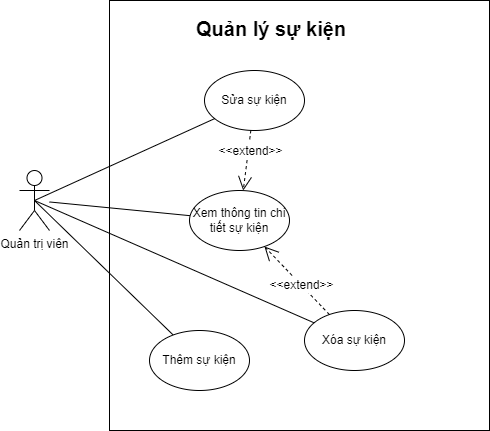
\includegraphics[width=8cm]{img/UseCase/UseCase-Quản lý sự kiện.drawio.png}
    \newline
    \caption{Use case quản lý sự kiện}
\end{figure}
\subsubsection{Xem thông tin chi tiết sự kiện}
\begin{longtable}{| p{.20\textwidth} | p{.80\textwidth} |} 
\hline
\textbf{Use-case name} 
& 
Xem thông tin chi tiết sự kiện.
\\
\hline
\textbf{Actor} 
& 
Quản trị viên
\\
\hline
\textbf{Description} 
& 
Cho phép quản trị viên xem  thông tin chi tiết sự kiện trong hệ thống.
\\
\hline
\textbf{Preconditions} 
&
Quản trị viên đã đăng nhập thành công vào hệ thống.
\\
\hline
\textbf{Postconditions} 
& 
Quản trị viên xem được được thông tin chi tiết của sự kiện mà họ muốn.
\\
\hline
\textbf{Trigger} 
& 
Quản trị viên chọn mục "sự kiện".
\\
\hline
\begin{flushleft}
\textbf{Normal flow}
\end{flushleft}
& 
1. Toàn bộ sự kiện được hiển thị lên trình duyệt.

    2.  Quản trị viên chọn sự kiện muốn xem thông tin chi tiết và nhấp chuột vào sự kiện đó.
    
3.  Hệ thống hiển thị thông tin chi tiết của sự kiện.

4. Người dùng xem thông tin chi tiết của sự kiện.
\\
\hline
\textbf{Alternative flow}
& 
Không.
%%%%%%%%%%%%%%%%
\\
\hline
\textbf{Exceptions} 
&
Không.
%%%%%%%%%%%%%%%%%%%%
\\
\hline
\caption{Đặc tả use-case \textbf{xem thông tin chi tiết sự kiện}}
\end{longtable}
\subsubsection{Thêm sự kiện cho hệ thống bán hàng online.}
\begin{longtable}{| p{.20\textwidth} | p{.80\textwidth} |} 
\hline
\textbf{Use-case name} 
& 
Thêm sự kiện cho hệ thống bán hàng online
\\
\hline
\textbf{Actor} 
& 
Quản trị viên
\\
\hline
\textbf{Description} 
& 
Cho phép quản trị viên có thể thêm sự kiện mới cho hệ thống bán hàng online.
\\
\hline
\textbf{Preconditions} 
&
Quản trị viên đã đăng nhập thành công vào hệ thống.
\\
\hline
\textbf{Postconditions} 
& 
Quản trị viên tạo mới được sự kiện mà họ muốn.
\\
\hline
\textbf{Trigger} 
& 
Quản trị viên chọn mục "sự kiện".
\\
\hline
\begin{flushleft}
\textbf{Normal flow}
\end{flushleft}
& 
    1. Toàn bộ sự kiện được hiển thị lên trình duyệt.
    
    2. Quản trị viên chọn nút thêm sự kiện.
    
    3. Hệ thống hiển thị màn hình form để tạo sự kiện mới
    .
    4. Quản trị viên nhập các thông tin cần thiết mà hệ thống yêu cầu và chọn icon "Thêm sự kiện".
    
    5. Hệ thống cập nhật thêm sự kiện mới vào database.
\\
\hline
\begin{flushleft}
\textbf{Alternative flow}
\end{flushleft}
& 
4.1. Người dùng không muốn tiếp tục nữa.
    \begin{quote}
        4.1.1. Người dùng chọn "Hủy".
        
        4.1.2. Hệ thống tắt màn hình popup.
    \end{quote}
%%%%%%%%%%%%%%%%
\\
\hline
\begin{flushleft}
\textbf{Exceptions} 
\end{flushleft}
&
5.1. Tên sự kiện đã tồn tại.
    \begin{quote}
        5.1.1. Hệ thống thông báo thêm sự kiện thất bại.
        
    5.1.2. Trở về bước 4.
    \end{quote}

%%%%%%%%%%%%%%%%%%%%
\\
\hline
\caption{Đặc tả use-case \textbf{thêm sự kiện cho hệ thống bán hàng online}}
\end{longtable}
            
\subsubsection{Chỉnh sửa sự kiện}
\begin{longtable}{| p{.20\textwidth} | p{.80\textwidth} |} 
\hline
\textbf{Use-case name} 
& 
Chỉnh sửa thông tin sự kiện
\\
\hline
\textbf{Actor} 
& 
Quản trị viên
\\
\hline
\textbf{Description} 
& 
Cho phép quản trị viên có thể chỉnh sửa thông tin sự kiện mới cho hệ thống bán hàng online.
\\
\hline
\textbf{Preconditions} 
&
Quản trị viên đã đăng nhập thành công vào hệ thống.
\\
\hline
\textbf{Postconditions} 
& 
Quản trị viên chỉnh sửa được sự kiện mà họ muốn.
\\
\hline
\textbf{Trigger} 
& 
Quản trị viên chọn mục "sự kiện".
\\
\hline
\begin{flushleft}
\textbf{Normal flow}
\end{flushleft}
& 
    1.Toàn bộ sự kiện được hiển thị lên trình duyệt.
    
    2. Quản trị viên chọn sự kiện muốn chỉnh sửa và nhấn vào nút "chỉnh sửa".
    
    3. Hệ thống hiển thị màn hình các thông tin của sự kiện.
    
    4. Quản trị viên chỉnh sửa các thông tin mà họ muốn sau đó nhấn nút "Lưu".
    
    5. Hệ thống thông báo kết quả cập nhật thêm sự kiện mới vào database.
\\
\hline
\begin{flushleft}
\textbf{Alternative flow}
\end{flushleft}
& 
4.1. Người dùng không muốn tiếp tục nữa.
    \begin{quote}
    4.1.1. Người dùng chọn "Hủy".
    
        4.1.2. Hệ thống tắt màn hình popup.
    \end{quote}
%%%%%%%%%%%%%%%%
\\
\hline
\begin{flushleft}
\textbf{Exceptions} 
\end{flushleft}
&
5.1. Thông tin thay đổi không hợp lệ
    \begin{quote} 
    5.1.1. Hệ thống thông báo chỉnh sửa sự kiện thất bại
    
    5.1.2. Trở về bước 4.
    \end{quote}
%%%%%%%%%%%%%%%%%%%%
\\
\hline
\caption{Đặc tả use-case \textbf{chỉnh sửa thông tin sự kiện}}
\end{longtable}
            
\subsubsection{Xóa sự kiện} 
\begin{longtable}
{| p{.20\textwidth} | p{.80\textwidth} |} 
\hline
\textbf{Use-case name} 
& 
Xóa sự kiện
\\
\hline
\textbf{Actor} 
& 
Quản trị viên
\\
\hline
\textbf{Description} 
& 
Cho phép quản trị viên có thể xóa sự kiện khi không muốn nữa.
\\
\hline
\textbf{Preconditions} 
&
Quản trị viên đã đăng nhập thành công vào hệ thống.
\\
\hline
\textbf{Postconditions} 
& 
Quản trị viên xóa được sự kiện mà họ muốn.
\\
\hline
\textbf{Trigger} 
& 
Quản trị viên chọn mục "sự kiện".
\\
\hline
\begin{flushleft}
\textbf{Normal flow}
\end{flushleft}
& 
1. Toàn bộ sự kiện được hiển thị lên trình duyệt.
    
    2. Quản trị viên chọn sự kiện muốn chỉnh sửa và nhấn vào nút "xóa".
    
    3. Hệ thống hiển thị màn hình xác nhận người dùng muốn xóa sự kiện.
    
    4. Quản trị viên chọn "Xác nhận".
\\
\hline
\begin{flushleft}
\textbf{Alternative flow}
\end{flushleft}
& 
4.1. Người dùng không muốn tiếp tục.
    \begin{quote}
    4.1.1. Người dùng chọn "Hủy".
    
    4.1.2.  Hệ thống tắt màn hình popup.
    \end{quote}
%%%%%%%%%%%%%%%%
\\
\hline
\begin{flushleft}
\textbf{Exceptions} 
\end{flushleft}
&
5.1.  Xóa sự kiện thất bại
    \begin{quote} 
    5.1.1. Hệ thống thông báo không thể xóa sự kiện.
    
    5.1.2. Trở về bước 2.
    \end{quote}
%%%%%%%%%%%%%%%%%%%%
\\
\hline
\caption{Đặc tả use-case \textbf{xóa sự kiện}}
\end{longtable}
            
    \subsection{Quản lý chi nhánh}
        \begin{figure}[!htp]
            \centering
            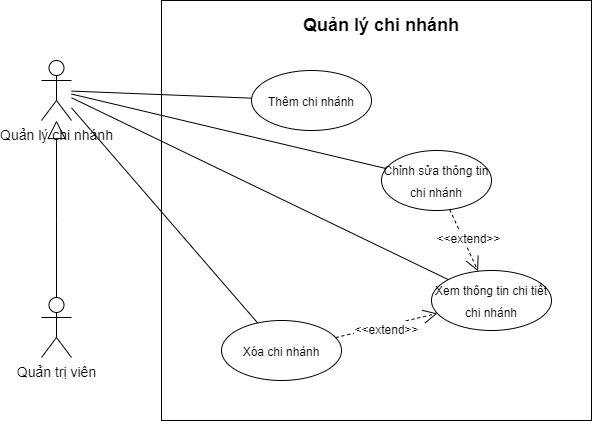
\includegraphics[width=9cm]{img/UseCase/UseCase-Quản lý chi nhánh.drawio.png}
            \newline
         \caption{Use case quản lý chi nhánh}
        \end{figure}
        \subsubsection{Thêm chi nhánh}
            \begin{longtable}{| p{.20\textwidth} | p{.80\textwidth} |}
                \hline
                    \textbf{Use-case name}
                &
                    Thêm chi nhánh
                \\
                %%%%%%%%%%%%%%%%
                \hline
                    \textbf{Actor}
                &
                    Quản lý chi nhánh
                \\
                %%%%%%%%%%%%%%%%
                \hline
                    \textbf{Description}
                &
                    Quản lý chi nhánh có thể thêm chi nhánh mới
                \\
                %%%%%%%%%%%%%%%%
                \hline
                    \textbf{Preconditions}
                &
                    Quản lý chi nhánh đã đăng nhập
                \\
                %%%%%%%%%%%%%%%%
                \hline
                    \textbf{Postconditions}
                &
                    Chi nhánh mới được cập nhật
                \\
                %%%%%%%%%%%%%%%%
                \hline
                    \textbf{Trigger}
                &
                    Quản lý chi nhánh chọn vào quản lý chi nhánh
                \\
                %%%%%%%%%%%%%%%%
                \hline
                \begin{flushleft}
                    \textbf{Normal flow}
                \end{flushleft}
                &
                1. Hệ thống hiển thị danh sách chi nhánh
                   
                    2. Quản lý chi nhánh chọn thêm mới
                   
                    3. Hệ thống hiển thị biểu mẫu nhập thông tin
                   
                    4. Quản trị viên nhập thông tin chi nhánh mới
                   
                    5. Quản trị viên nhập chọn xác nhận
                   
                    6. Hệ thống cập nhật chi nhánh mới
                \\
                %%%%%%%%%%%%%%%%
                \hline
                \begin{flushleft}
                    \textbf{Alternative flow}
                \end{flushleft}
                &
                5.1. Quản trị viên nhập chọn hủy
                    \begin{quote}
                    5.1.1. Kết thúc
                    \end{quote}
                \\
                %%%%%%%%%%%%%%%%
                \hline
                \begin{flushleft}
                    \textbf{Exceptions}
                \end{flushleft}
                &
                6.1. Tên chi nhánh bị trùng
                    \begin{quote}
                    6.1.1. Quay về bước 3
                    \end{quote}
                \\
                \hline
                 %%%%%%%%%%%%%%%%
                \caption{Đặc tả use-case \textbf{thêm chi nhánh}}
            \end{longtable}
           
        \subsubsection{Chỉnh sửa thông tin chi nhánh}
            \begin{longtable}{| p{.20\textwidth} | p{.80\textwidth} |}
                \hline
                    \textbf{Use-case name}
                &
                    Chỉnh sửa tin chi nhánh
                \\
                %%%%%%%%%%%%%%%%
                \hline
                    \textbf{Actor}
                &
                    Quản lý chi nhánh
                \\
                %%%%%%%%%%%%%%%%
                \hline
                    \textbf{Description}
                &
                    Quản lý chi nhánh có thể chỉnh sửa thông tin chi nhánh
                \\
                %%%%%%%%%%%%%%%%
                \hline
                    \textbf{Preconditions}
                &
                    Quản lý chi nhánh đã đăng nhập
                \\
                %%%%%%%%%%%%%%%%
                \hline
                    \textbf{Postconditions}
                &
                    Thông tin chi nhánh được cập nhật
                \\
                %%%%%%%%%%%%%%%%
                \hline
                    \textbf{Trigger}
                &
                    Quản lý chi nhánh chọn vào quản lý chi nhánh
                \\
                %%%%%%%%%%%%%%%%
                \hline
                \begin{flushleft}
                    \textbf{Normal flow}
                \end{flushleft}
                &
                1. Hệ thống hiển thị danh sách chi nhánh
               
                    2. Quản lý chi nhánh tìm kiếm chi nhánh và chọn chỉnh sửa
                   
                    3. Hệ thống hiển thị biểu mẫu nhập thông tin
                   
                    4. Quản lý chi nhánh chỉnh sửa thông tin chi nhánh
                   
                    5. Quản lý chi nhánh nhập chọn xác nhận
                   
                    6. Hệ thống cập nhật thông tin  chi nhánh
                \\
                %%%%%%%%%%%%%%%%
                \hline
                \begin{flushleft}
                    \textbf{Alternative flow}
                \end{flushleft}
                &
                5.1. Quản lý chi nhánh chọn hủy
                    \begin{quote}
                    5.1.1. Kết thúc
                    \end{quote}
                \\
                %%%%%%%%%%%%%%%%
                \hline
                \begin{flushleft}
                    \textbf{Exceptions}
                \end{flushleft}
                &
                6.1. Tên chi nhánh bị trùng
                    \begin{quote}
                    6.1.1. Quay về bước 3
                    \end{quote}
                \\
                \hline
                 %%%%%%%%%%%%%%%%
                \caption{Đặc tả use-case \textbf{chỉnh sửa chi nhánh}}
            \end{longtable}
           
        \subsubsection{Xem thông tin chi tiết chi nhánh}
            \begin{longtable}{| p{.20\textwidth} | p{.80\textwidth} |}
                \hline
                    \textbf{Use-case name}
                &
                    Xem thông tin chi tiết chi nhánh
                \\
                %%%%%%%%%%%%%%%%
                \hline
                    \textbf{Actor}
                &
                    Quản lý chi nhánh
                \\
                %%%%%%%%%%%%%%%%
                \hline
                    \textbf{Description}
                &
                    Quản lý chi nhánh có thể xem thông tin chi nhánh
                \\
                %%%%%%%%%%%%%%%%
                \hline
                    \textbf{Preconditions}
                &
                    Quản lý chi nhánh đã đăng nhập
                \\
                %%%%%%%%%%%%%%%%
                \hline
                    \textbf{Postconditions}
                &
                    Nhận được thông tin chi nhánh
                \\
                %%%%%%%%%%%%%%%%
                \hline
                    \textbf{Trigger}
                &
                    Quản lý chi nhánh truy cập quản lý chi nhánh
                \\
                %%%%%%%%%%%%%%%%
                \hline
                \begin{flushleft}
                    \textbf{Normal flow}
                \end{flushleft}
                &
                1. Hệ thống hiển thị danh sách các chi nhánh
               
                    2. Quản lý chi nhánh tìm kiếm và chọn chi nhánh muốn xem
                   
                    3. Hệ thống hiển thị thông tin chi nhánh đã chọn
                \\
                %%%%%%%%%%%%%%%%
                \hline
                    \textbf{Alternative flow}
                &
                    Không
                \\
                %%%%%%%%%%%%%%%%
                \hline
                    \textbf{Exceptions}
                &
                    Không
                \\
                \hline
                 %%%%%%%%%%%%%%%%
                \caption{Đặc tả use-case \textbf{xem thông tin chi tiết chi nhánh}}
            \end{longtable}
           
        \subsubsection{Xóa chi nhánh}
            \begin{longtable}{| p{.20\textwidth} | p{.80\textwidth} |}
                \hline
                    \textbf{Use-case name}
                &
                    Xóa chi nhánh
                \\
                %%%%%%%%%%%%%%%%
                \hline
                    \textbf{Actor}
                &
                    Quản lý chi nhánh
                \\
                %%%%%%%%%%%%%%%%
                \hline
                    \textbf{Description}
                &
                    Quản lý chi nhánh có thể xóa chi nhánh
                \\
                %%%%%%%%%%%%%%%%
                \hline
                    \textbf{Preconditions}
                &
                    Quản lý chi nhánh đã đăng nhập
                \\
                %%%%%%%%%%%%%%%%
                \hline
                    \textbf{Postconditions}
                &
                    Chi nhánh bị xóa khỏi hệ thống
                \\
                %%%%%%%%%%%%%%%%
                \hline
                    \textbf{Trigger}
                &
                    Quản lý chi nhánh chọn quản lý chi nhánh            
                \\
                %%%%%%%%%%%%%%%%
                \hline
                \begin{flushleft}
                    \textbf{Normal flow}
                \end{flushleft}
                &
                1. Hệ thống hiển thị danh sách chi nhánh
               
                    2. Quản lý chi nhánh tìm và chọn chi nhánh muốn xóa
                   
                  3. Hệ thống hiển thị thông tin chi tiết chi nhánh
 
                    4. Quản lý chi nhánh chọn xóa chi nhánh
                   
                    5. Hệ thống yêu cầu xác nhận
                   
                    6. Quản lý chi nhánh chọn xác nhận
                   
                    7. Hệ thống cập nhật thông tin
                \\
                %%%%%%%%%%%%%%%%
                \hline
                \begin{flushleft}
                    \textbf{Alternative flow}
                \end{flushleft}
                &
                6.1. Quản trị viên chọn hủy
                    \begin{quote}
                    6.1.1. Quay lại bước 3
                    \end{quote}
                \\
                %%%%%%%%%%%%%%%%
                \hline
                    \textbf{Exceptions}
                &
                    Không
                \\
                \hline
                 %%%%%%%%%%%%%%%%
                \caption{Đặc tả use-case \textbf{xóa chi nhánh}}
            \end{longtable}
        

    \subsection{Quản lý hoạt động kinh doanh}
        \begin{figure}[!htp]
            \centering
            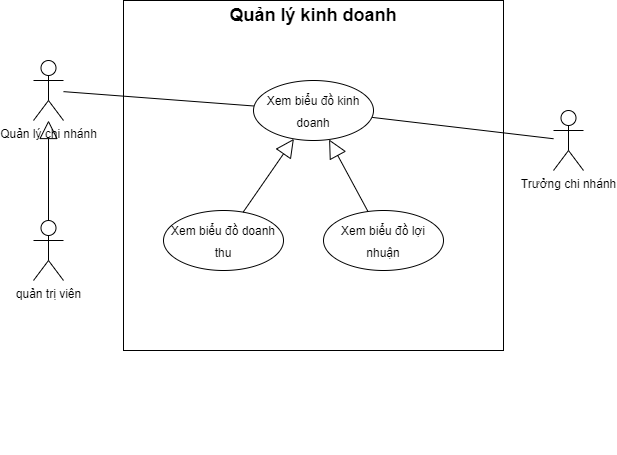
\includegraphics[width=8cm]{img/UseCase/UseCase-Quản lý hoạt động kinh doanh.drawio.png}
            \newline
            \caption{Use case quản lý hoạt động kinh doanh}
        \end{figure}
        \subsubsection{Xem biểu đồ kinh doanh}
            \begin{longtable}{| p{.20\textwidth} | p{.80\textwidth} |} 
                \hline
                    \textbf{Use-case name} 
                & 
                    Xem biểu đồ kinh doanh 
                \\
                %%%%%%%%%%%%%%%%
                \hline
                    \textbf{Actor} 
                & 
                    Quản lý chi nhánh, trưởng chi nhánh
                \\
                %%%%%%%%%%%%%%%%
                \hline
                    \textbf{Description} 
                & 
                    Quản lý chi nhánh, trưởng chi nhánh có thể xem biểu đồ kinh doanh
                \\
                %%%%%%%%%%%%%%%%
                \hline
                    \textbf{Preconditions} 
                &
                    Quản lý chi nhánh, trưởng chi nhánh đã đăng nhập
                \\
                %%%%%%%%%%%%%%%%
                \hline
                    \textbf{Postconditions} 
                & 
                    Nhận được biểu đồ kinh doanh
                \\
                %%%%%%%%%%%%%%%%
                \hline
                    \textbf{Trigger} 
                & 
                    Quản lý chi nhánh, trưởng chi nhánh chọn quản lý hoạt động kinh doanh      
                \\
                %%%%%%%%%%%%%%%%
                \hline
                \begin{flushleft}
                    \textbf{Normal flow}
                \end{flushleft}
                & 
                1. Quản lý chi nhánh, trưởng chi nhánh loại hàng muốn thống kê
                    
                    2. Quản lý chi nhánh, trưởng chi nhánh chọn khoảng thời gian 
                    
                    3. Quản lý chi nhánh, trưởng chi nhánh chọn loại biểu đồ
                    
                    4. Hệ thống hiển thị biểu đồ
                \\
                %%%%%%%%%%%%%%%%
                \hline
                    \textbf{Alternative flow}
                &
                    Không
                \\
                %%%%%%%%%%%%%%%%
                \hline
                    \textbf{Exceptions} 
                &
                    Không
                \\
                \hline
                 %%%%%%%%%%%%%%%%
                \caption{Đặc tả use-case \textbf{xem biểu đồ kinh doanh}}
            \end{longtable}


    \subsection{Quản lý nhân viên}    
        \begin{figure}[!htp]
            \begin{center}
                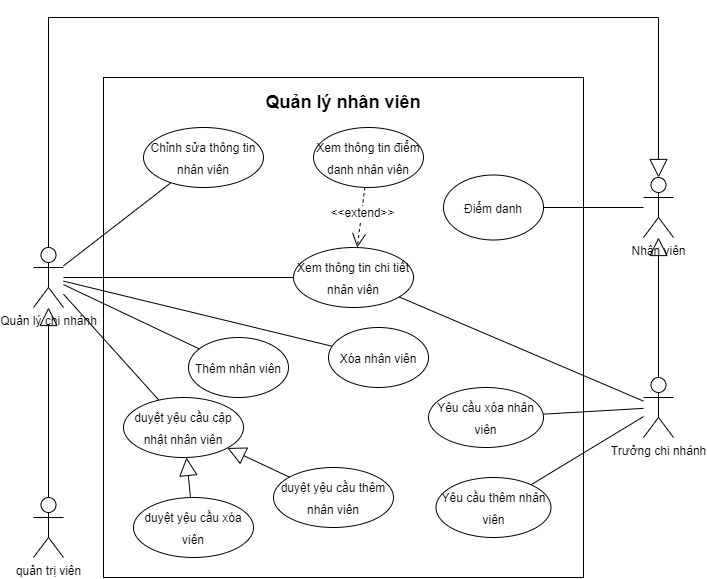
\includegraphics[width=10cm]{img/UseCase/UseCase-Quản lý nhân viên.drawio.png}
            \end{center}
            \caption{Use case quản lý nhân viên}
        \end{figure}


        \subsubsection{Xem thông tin chi tiết nhân viên}
            \begin{longtable}{| p{.20\textwidth} | p{.80\textwidth} |} 
                \hline
                    \textbf{Use-case name} 
                & 
                    Xem thông tin chi tiết nhân viên
                \\
                %%%%%%%%%%%%%%%%%%
                \hline
                    \textbf{Actor} 
                & 
                    Quản lý chi nhánh, trưởng chi nhánh
                \\
                %%%%%%%%%%%%%%%%%%
                \hline
                    \textbf{Description} 
                & 
                    Quản lý chi nhánh, trưởng chi nhánh có thể xem thông tin chi tiết nhân viên
                \\
                %%%%%%%%%%%%%%%%%%
                \hline
                    \textbf{Preconditions} 
                &
                    Quản lý chi nhánh, trưởng chi nhánh đã đăng nhập
                \\
                %%%%%%%%%%%%%%%%%%
                \hline
                    \textbf{Postconditions} 
                & 
                    Nhận được thông tin chi tiết nhân viên
                \\
                %%%%%%%%%%%%%%%%%%
                \hline
                    \textbf{Trigger} 
                & 
                    Quản lý chi nhánh, trưởng chi nhánh chọn quản lý nhân viên
                \\
                %%%%%%%%%%%%%%%%%%
                \hline
                \begin{flushleft}
                    \textbf{Normal flow}
                \end{flushleft}
                & 
                1. Hệ thống hiển thị danh sách nhân viên
                
                    2. Quản lý chi nhánh, trưởng chi nhánh tìm và chọn nhân viên muốn xem
                    
                    3. Hệ thống hiển thị thông tin chi tiết nhân viên
                \\
                %%%%%%%%%%%%%%%%%%
                \hline
                    \textbf{Alternative flow}
                &
                    Không
                \\
                %%%%%%%%%%%%%%%%%%
                \hline
                    \textbf{Exceptions} 
                &
                    Không
                \\
                %%%%%%%%%%%%%%%%%%
                \hline
                \caption{Đặc tả use-case \textbf{xem thông tin chi tiết nhân viên}}
            \end{longtable}

        \newpage
        \subsubsection{Xem thông tin điểm danh nhân viên}
            \begin{longtable}{| p{.20\textwidth} | p{.80\textwidth} |} 
                \hline
                    \textbf{Use-case name} 
                & 
                    Xem thông tin điểm danh nhân viên
                \\
                %%%%%%%%%%%%%%%%%%
                \hline
                    \textbf{Actor} 
                & 
                    Quản lý chi nhánh, trưởng chi nhánh
                \\
                %%%%%%%%%%%%%%%%%%
                \hline
                    \textbf{Description} 
                & 
                    Quản lý chi nhánh, trưởng chi nhánh có thể xem thông tin điểm danh nhân viên
                \\
                %%%%%%%%%%%%%%%%%%
                \hline
                    \textbf{Preconditions} 
                &
                    Quản lý chi nhánh, trưởng chi nhánh đã đăng nhập 
                \\
                %%%%%%%%%%%%%%%%%%
                \hline
                    \textbf{Postconditions} 
                & 
                    Nhận được thông tin điểm danh nhân viên
                \\
                %%%%%%%%%%%%%%%%%%
                \hline
                    \textbf{Trigger} 
                & 
                    Quản lý chi nhánh, trưởng chi nhánh truy cập thông tin chi tiết nhân viên
                \\
                %%%%%%%%%%%%%%%%%%
                \hline
                \begin{flushleft}
                    \textbf{Normal flow}
                \end{flushleft}
                & 
                1. Hệ thống hiển thị thông tin chi tiết nhân viên
                
                    2. Quản lý chi nhánh, trưởng chi nhánh chọn thời gian muốn xem
                    
                    3. Hệ thống hiển thị lịch điểm danh nhân viên
                \\
                %%%%%%%%%%%%%%%%%%
                \hline
                    \textbf{Alternative flow}
                &
                    Không
                \\
                %%%%%%%%%%%%%%%%%%
                \hline
                    \textbf{Exceptions} 
                &
                    Không
                \\
                %%%%%%%%%%%%%%%%%%
                \hline
                \caption{Đặc tả use-case \textbf{xem thông tin chi tiết nhân viên}}
            \end{longtable}
    
        \subsubsection{Chỉnh sửa thông tin chi tiết nhân viên}
            \begin{longtable}{| p{.20\textwidth} | p{.80\textwidth} |} 
                \hline
                    \textbf{Use-case name} 
                & 
                    Chỉnh sửa thông tin chi tiết nhân viên
                \\
                %%%%%%%%%%%%%%%%%%
                \hline
                    \textbf{Actor} 
                & 
                    Quản lý chi nhánh
                \\
                %%%%%%%%%%%%%%%%%%
                \hline
                    \textbf{Description} 
                & 
                    Quản lý chi nhánh có thể chỉnh sửa thông tin nhân viên.
                \\
                %%%%%%%%%%%%%%%%%%
                \hline
                    \textbf{Preconditions} 
                &
                    Quản lý chi nhánh đã đăng nhập
                \\
                %%%%%%%%%%%%%%%%%%
                \hline
                    \textbf{Postconditions} 
                & 
                    Thông tin nhân viên được cập nhật
                \\
                %%%%%%%%%%%%%%%%%%
                \hline
                    \textbf{Trigger} 
                & 
                    Quản lý chi nhánh chọn quản lý nhân viên
                \\
                %%%%%%%%%%%%%%%%%%
                \hline
                \begin{flushleft}
                    \textbf{Normal flow}
                \end{flushleft}
                & 
                1. Hệ thống hiển thị danh sách  nhân viên
                    
                    2. Quản lý chi nhánh tìm và chọn nhân viên cần chỉnh sửa
                    
                    3. Hệ thống hiển thị biểu mẫu thông tin nhân viên
                    
                    4. Quản lý chỉnh sửa thông tin
                    
                    5. Quản lý chọn lưu
                    
                    6. Hệ thống cập nhật thông tin
                \\
                %%%%%%%%%%%%%%%%%%
                \hline
                \begin{flushleft}
                    \textbf{Alternative flow}
                \end{flushleft}
                &
                5.1. Quản lý chọn hủy
                    \begin{quote} 
                    5.1.1. Quay lại bước 3
                    \end{quote}
                \\
                %%%%%%%%%%%%%%%%%%
                \hline
                    \textbf{Exceptions} 
                &
                    Không
                \\
                %%%%%%%%%%%%%%%%%%
                \hline
                \caption{Đặc tả use-case \textbf{chỉnh sửa thông tin nhân viên}}
            \end{longtable}
    
        \subsubsection{Thêm nhân viên}
            \begin{longtable}{| p{.20\textwidth} | p{.80\textwidth} |} 
                \hline
                    \textbf{Use-case name} 
                & 
                    Thêm nhân viên
                \\
                %%%%%%%%%%%%%%%%%%
                \hline
                    \textbf{Actor} 
                & 
                    Quản lý chi nhánh
                \\
                %%%%%%%%%%%%%%%%%%
                \hline
                    \textbf{Description} 
                & 
                    Quản lý chi nhánh có thể thêm nhân viên
                \\
                %%%%%%%%%%%%%%%%%%
                \hline
                    \textbf{Preconditions} 
                &
                    Quản lý chi nhánh đã đăng nhập
                \\
                %%%%%%%%%%%%%%%%%%
                \hline
                    \textbf{Postconditions} 
                & 
                    Thông tin nhân viên mới được cập nhật
                \\
                %%%%%%%%%%%%%%%%%%
                \hline
                    \textbf{Trigger} 
                & 
                    Quản lý chi nhánh chọn quản lý nhân viên
                \\
                %%%%%%%%%%%%%%%%%%
                \hline
                \begin{flushleft}
                    \textbf{Normal flow}
                \end{flushleft}
                & 
                1. Hệ thống hiển thị danh sách nhân viên
                    
                    2. Quản lý chi nhánh chọn thêm mới
                    
                    3. Hệ thống hiển thị biểu mẫu thông tin  nhân viên mới
                    
                    4. Quản lý chi nhánh nhập thông tin nhân viên
                    
                    5. Quản lý chi nhánh chọn lưu
                    
                    6. Hệ thống cập nhật thông tin
                \\
                %%%%%%%%%%%%%%%%%%
                \hline
                \begin{flushleft}
                    \textbf{Alternative flow}
                \end{flushleft}
                &
                5.1. Quản lý chọn hủy
                    \begin{quote} 
                    5.1.1. Quay lại bước 3
                    \end{quote}
                \\
                %%%%%%%%%%%%%%%%%%
                \hline
                    \textbf{Exceptions} 
                &
                    Không
                \\
                %%%%%%%%%%%%%%%%%%
                \hline
                \caption{Đặc tả use-case \textbf{Thêm nhân viên}}
            \end{longtable}
    
        \subsubsection{Xóa nhân viên}
            \begin{longtable}{| p{.20\textwidth} | p{.80\textwidth} |} 
                \hline
                    \textbf{Use-case name} 
                & 
                    Xóa nhân viên
                \\
                %%%%%%%%%%%%%%%%%%
                \hline
                    \textbf{Actor} 
                & 
                    Quản lý chi nhánh
                \\
                %%%%%%%%%%%%%%%%%%
                \hline
                    \textbf{Description} 
                & 
                    Quản lý chi nhánh có thể xóa nhân viên
                \\
                %%%%%%%%%%%%%%%%%%
                \hline
                    \textbf{Preconditions} 
                &
                    Quản lý chi nhánh đã đăng nhập
                \\
                %%%%%%%%%%%%%%%%%%
                \hline
                    \textbf{Postconditions} 
                & 
                    Thông tin nhân viên được xóa
                \\
                %%%%%%%%%%%%%%%%%%
                \hline
                    \textbf{Trigger} 
                & 
                    Quản lý chi nhánh chọn quản lý nhân viên
                \\
                %%%%%%%%%%%%%%%%%%
                \hline
                \begin{flushleft}
                    \textbf{Normal flow}
                \end{flushleft}
                & 
                    1. Hệ thống hiển thị danh sách nhân viên
                    
                    2. Quản lý chi nhánh tìm và chọn nhân viên muốn xóa
                    
                    3. Hệ thống hiển thị thông tin chi tiết nhân viên
                    
                    4. Quản lý chi nhánh chọn xóa
                    
                    5. Hệ thống yêu cầu xác nhận
                    
                    6. Quản lý chi nhánh chọn xác nhận
                    
                    7. Hệ thống cập nhật thông tin
                \\
                %%%%%%%%%%%%%%%%%%
                \hline
                    \textbf{Alternative flow}
                &
                    6.1. Quản lý chọn hủy
                    \begin{quote}
                        6.1.1. Quay lại bước 3
                    \end{quote} 
                \\
                %%%%%%%%%%%%%%%%%%
                \hline
                    \textbf{Exceptions} 
                &
                    Không
                \\
                %%%%%%%%%%%%%%%%%%
                \hline
                \caption{Đặc tả use-case \textbf{Xóa nhân viên}}
            \end{longtable}
    
 
        \subsubsection{Yêu cầu thêm nhân viên}
            \begin{longtable}{| p{.20\textwidth} | p{.80\textwidth} |} 
                \hline
                    \textbf{Use-case name} 
                & 
                    Yêu cầu thêm nhân viên
                \\
                %%%%%%%%%%%%%%%%%%
                \hline
                    \textbf{Actor} 
                & 
                    Trưởng chi nhánh
                \\
                %%%%%%%%%%%%%%%%%%
                \hline
                    \textbf{Description} 
                & 
                    Trưởng chi nhánh có thể yêu cầu cấp trên thêm nhân viên.
                \\
                %%%%%%%%%%%%%%%%%%
                \hline
                    \textbf{Preconditions} 
                &
                    Trưởng chi nhánh đã đăng nhập
                \\
                %%%%%%%%%%%%%%%%%%
                \hline
                    \textbf{Postconditions} 
                & 
                    Yêu cầu thêm được gửi đi
                \\
                %%%%%%%%%%%%%%%%%%
                \hline
                    \textbf{Trigger} 
                & 
                    Trưởng chi nhánh chọn vào quản lý nhân viên
                \\
                %%%%%%%%%%%%%%%%%%
                \hline
                \begin{flushleft}
                    \textbf{Normal flow}
                \end{flushleft}
                & 
                1. Hệ thống hiển thị danh sách nhân viên
                    
                    2. Trưởng chi nhánh chọn yêu cầu thêm mới
                    
                    3. Hệ thống hiển thị biểu mẫu nhập thông tin
                    
                    4. Trưởng chi nhánh nhập thông tin
                    
                    5. Trưởng chi nhánh chọn gửi
                    
                    6. Hệ thống gửi yêu cầu
                \\
                %%%%%%%%%%%%%%%%%%
                \hline
                    \textbf{Alternative flow}
                &
                    Không
                \\
                %%%%%%%%%%%%%%%%%%
                \hline
                    Không
                &
                    Không
                \\
                %%%%%%%%%%%%%%%%%%
                \hline
                \caption{Đặc tả use-case \textbf{Yêu cầu thêm nhân viên}}
            \end{longtable}
        
        \subsubsection{Yêu cầu xóa nhân viên}
            \begin{longtable}{| p{.20\textwidth} | p{.80\textwidth} |} 
                \hline
                    \textbf{Use-case name} 
                & 
                    Yêu cầu xóa nhân viên
                \\
                %%%%%%%%%%%%%%%%%%
                \hline
                    \textbf{Actor} 
                & 
                    Trưởng chi nhánh
                \\
                %%%%%%%%%%%%%%%%%%
                \hline
                    \textbf{Description} 
                & 
                    Trưởng chi nhánh có thể yêu cầu cấp trên xóa nhân viên.
                \\
                %%%%%%%%%%%%%%%%%%
                \hline
                    \textbf{Preconditions} 
                &
                    Trưởng chi nhánh đã đăng nhập
                \\
                %%%%%%%%%%%%%%%%%%
                \hline
                    \textbf{Postconditions} 
                & 
                    Yêu cầu xóa được gửi đi
                \\
                %%%%%%%%%%%%%%%%%%
                \hline
                    \textbf{Trigger} 
                & 
                    Trưởng chi nhánh chọn quản lý nhân viên
                \\
                %%%%%%%%%%%%%%%%%%
                \hline
                \begin{flushleft}
                    \textbf{Normal flow}
                \end{flushleft}
                & 
                1. Hệ thống hiển thị danh sách nhân viên
                    
                    2. Trưởng chi nhánh tìm và chọn nhân viên muốn yêu cầu
                    
                    3. Hệ thống hiển thị thông tin nhân viên
                    
                    4. Trưởng chi nhánh chọn yêu cầu xóa
                    
                    5. Hệ thống gửi thông tin đi
                \\
                %%%%%%%%%%%%%%%%%%
                \hline
                    \textbf{Alternative flow}
                &
                    Không
                \\
                %%%%%%%%%%%%%%%%%%
                \hline
                    \textbf{Exceptions} 
                &
                    Không
                \\
                %%%%%%%%%%%%%%%%%%
                \hline
                \caption{Đặc tả use-case \textbf{Yêu cầu xóa nhân viên}}
            \end{longtable}
        
        \subsubsection{Duyệt yêu cầu cập nhật nhân viên}
            \begin{longtable}{| p{.20\textwidth} | p{.80\textwidth} |} 
                \hline
                    \textbf{Use-case name} 
                & 
                    Duyệt yêu cầu thêm nhân viên
                \\
                %%%%%%%%%%%%%%%%%%
                \hline
                    \textbf{Actor} 
                & 
                    Quản lý chi nhánh
                \\
                %%%%%%%%%%%%%%%%%%
                \hline
                    \textbf{Description} 
                & 
                    Quản lý chi nhánh có thể thêm nhân viên từ yêu cầu
                \\
                %%%%%%%%%%%%%%%%%%
                \hline
                    \textbf{Preconditions} 
                &
                    Quản lý chi nhánh đã đăng nhập
                \\
                %%%%%%%%%%%%%%%%%%
                \hline
                    \textbf{Postconditions} 
                & 
                    Thông tin nhân viên được thêm
                \\
                %%%%%%%%%%%%%%%%%%
                \hline
                    \textbf{Trigger} 
                & 
                    Quản lý chi nhánh chọn quản lý nhân viên
                \\
                %%%%%%%%%%%%%%%%%%
                \hline
                \begin{flushleft}
                    \textbf{Normal flow}
                \end{flushleft}
                & 
                1. Hệ thống hiển thị danh sách nhân viên
                    
                    2. Quản lý chi nhánh chọn được yêu cầu
                    
                    3. Hệ thống hiển thị danh sách yêu cầu nhân viên đang chờ
                    
                    4. Quản lý chi nhánh tìm và chọn duyệt nhân viên được yêu cầu
                    
                    5. Hệ thống yêu cầu xác nhận
                    
                    6. Quản lý chi nhánh chọn xác nhận
                    
                    7. Hệ thống cập nhật thông tin
                \\
                %%%%%%%%%%%%%%%%%%
                \hline
                    \textbf{Alternative flow}
                &
                6.1. Quản lý chọn hủy
                    \begin{quote} 
                    6.1.1. Quay lại bước 3
                    \end{quote}
                \\
                %%%%%%%%%%%%%%%%%%
                \hline
                    \textbf{Exceptions} 
                &
                    Không
                \\
                %%%%%%%%%%%%%%%%%%
                \hline
                \caption{Đặc tả use-case \textbf{Duyệt yêu cầu cập nhật nhân viên}}
            \end{longtable}

        \subsubsection{Điểm danh}
            \begin{longtable}{| p{.20\textwidth} | p{.80\textwidth} |} 
                \hline
                    \textbf{Use-case name} 
                & 
                    Điểm danh
                \\
                %%%%%%%%%%%%%%%%%%
                \hline
                    \textbf{Actor} 
                & 
                    Nhân viên
                \\
                %%%%%%%%%%%%%%%%%%
                \hline
                    \textbf{Description} 
                & 
                    Nhân viên điểm danh khi làm việc
                \\
                %%%%%%%%%%%%%%%%%%
                \hline
                    \textbf{Preconditions} 
                &
                    Không
                \\
                %%%%%%%%%%%%%%%%%%
                \hline
                    \textbf{Postconditions} 
                & 
                    Nhân viên được điểm danh
                \\
                %%%%%%%%%%%%%%%%%%
                \hline
                    \textbf{Trigger} 
                & 
                    Nhân viên truy cập hệ thống điểm danh
                \\
                %%%%%%%%%%%%%%%%%%
                \hline
                    \textbf{Normal flow}
                & 
                1. Nhân viên đưa thẻ nhân viên vào máy scan
                    
                    2. Hệ thống quét và cập nhật thông tin
                \\
                %%%%%%%%%%%%%%%%%%
                \hline
                    \textbf{Alternative flow}
                &
                    Không
                \\
                %%%%%%%%%%%%%%%%%%
                \hline
                    \textbf{Exceptions} 
                &
                    Không
                \\
                %%%%%%%%%%%%%%%%%%
                \hline
                \caption{Đặc tả use-case \textbf{điểm danh}}
            \end{longtable}

   \newpage         
    
   
   \subsection{Quản lý tài khoản}
        \begin{figure}[!htp]
            \centering
            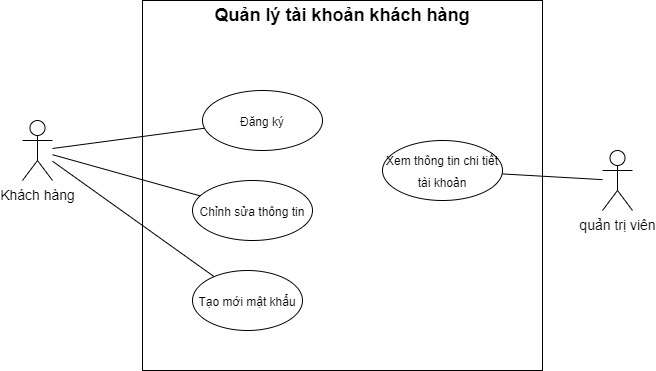
\includegraphics[width=9cm]{img/UseCase/UseCase-Quản lý tài khoản.drawio.png}
            \newline
         \caption{Use case quản lý tài khoản}
        \end{figure}
        
        \subsubsection{Đăng ký}
            \begin{longtable}{| p{.20\textwidth} | p{.80\textwidth} |} 
                \hline
                    \textbf{Use-case name} 
                & 
                    Đăng ký
                \\
                %%%%%%%%%%%%%%%%%%
                \hline
                    \textbf{Actor} 
                & 
                    Khách hàng
                \\
                %%%%%%%%%%%%%%%%%%
                \hline
                    \textbf{Description} 
                & 
                  Khách hàng có thể đăng ký tài khoản
                \\
                %%%%%%%%%%%%%%%%%%
                \hline
                    \textbf{Preconditions} 
                &
                    Khách hàng truy cập hệ thống
                \\
                %%%%%%%%%%%%%%%%%%
                \hline
                    \textbf{Postconditions} 
                & 
                    Tài khoản được đăng ký
                \\
                %%%%%%%%%%%%%%%%%%
                \hline
                    \textbf{Trigger} 
                & 
                    Khách hàng chọn đăng ký
                \\
                %%%%%%%%%%%%%%%%%%
                \hline
                \begin{flushleft}
                    \textbf{Normal flow}
                \end{flushleft}
                & 
                1. Hệ thống hiển thị biểu mẫu thông tin khách hàng
                    
                    2. Khách hàng nhập thông tin của mình
                    
                    3. Khách hạng chọn đăng ký
                    
                    4. Hệ thống hiện yêu cầu nhập mã xác nhận
                    
                    5. Khách hàng nhập mã và chọn gửi
                    
                    6. Hệ thống cập nhật thông tin
                \\
                %%%%%%%%%%%%%%%%%%
                \hline
                \begin{flushleft}
                    \textbf{Alternative flow}
                \end{flushleft}
                &
                3.1. Khách hàng chọn hủy
                    \begin{quote} 
                    3.1.1 Kết thúc
                    \end{quote}
                \\
                %%%%%%%%%%%%%%%%%%
                \hline
                \begin{flushleft}
                    \textbf{Exceptions} 
                \end{flushleft}
                &
                4.1. Số điện thoại đã được sử dụng
                    \begin{quote} 
                    4.1.1 Quay lại bước 1
                    \end{quote}
                6.1. Khách hàng nhập sai OTP
                    \begin{quote} 
                    6.1.1 Quay lại bước 5
                    \end{quote}
                \\
                %%%%%%%%%%%%%%%%%%
                \hline
                \caption{Đặc tả use-case \textbf{Đăng ký}}
            \end{longtable}
        
        \subsubsection{Chỉnh sửa thông tin}
            \begin{longtable}{| p{.20\textwidth} | p{.80\textwidth} |} 
                \hline
                    \textbf{Use-case name} 
                & 
                    Chỉnh sửa thông tin
                \\
                %%%%%%%%%%%%%%%%%%
                \hline
                    \textbf{Actor} 
                & 
                    Khách hàng
                \\
                %%%%%%%%%%%%%%%%%%
                \hline
                    \textbf{Description} 
                & 
                  Khách hàng có thể chỉnh sửa thông tin cá nhân
                \\
                %%%%%%%%%%%%%%%%%%
                \hline
                    \textbf{Preconditions} 
                &
                    Khách hàng đã đăng nhập
                \\
                %%%%%%%%%%%%%%%%%%
                \hline
                    \textbf{Postconditions} 
                & 
                    Thông tin được cập nhật
                \\
                %%%%%%%%%%%%%%%%%%
                \hline
                    \textbf{Trigger} 
                & 
                    Khách hàng chọn vào tài khoản
                \\
                %%%%%%%%%%%%%%%%%%
                \hline
                \begin{flushleft}
                    \textbf{Normal flow}
                \end{flushleft}
                & 
                1. Hệ thống hiển thị biểu mẫu thông tin tài khoản
                    
                    2. Khách hàng chỉnh sửa thông tin tài khoản
                    
                    3. Khách hàng chọn lưu
                    
                    4. Hệ thống cập nhật thông tin
                \\
                %%%%%%%%%%%%%%%%%%
                \hline
                \begin{flushleft}
                    \textbf{Alternative flow}
                \end{flushleft}
                &
                3.1.Khách hàng chọn hủy
                    \begin{quote} 
                    3.1.1 Kết thúc
                    \end{quote}
                \\
                %%%%%%%%%%%%%%%%%%
                \hline
                    \textbf{Exceptions} 
                &
                    Không
                \\
                %%%%%%%%%%%%%%%%%%
                \hline
                \caption{Đặc tả use-case \textbf{Chỉnh sửa thông tin}}
            \end{longtable}
 
        \subsubsection{Tạo mới mật khẩu}
            \begin{longtable}{| p{.20\textwidth} | p{.80\textwidth} |} 
                \hline
                    \textbf{Use-case name} 
                & 
                    Tạo mới mật khẩu
                \\
                %%%%%%%%%%%%%%%%%%
                \hline
                    \textbf{Actor} 
                & 
                    Khách hàng
                \\
                %%%%%%%%%%%%%%%%%%
                \hline
                    \textbf{Description} 
                & 
                  Khách hàng có thể cập nhật mật khẩu mới khi quên mật khẩu
                \\
                %%%%%%%%%%%%%%%%%%
                \hline
                    \textbf{Preconditions} 
                &
                    Khách hàng đã truy cập hệ thống
                \\
                %%%%%%%%%%%%%%%%%%
                \hline
                    \textbf{Postconditions} 
                & 
                    Thông tin được cập nhật
                \\
                %%%%%%%%%%%%%%%%%%
                \hline
                    \textbf{Trigger} 
                & 
                    Khách hàng chọn vào quên mật khẩu
                \\
                %%%%%%%%%%%%%%%%%%
                \hline
                \begin{flushleft}
                    \textbf{Normal flow}
                \end{flushleft}
                & 
                1. Hệ thống yêu cầu thông tin liên hệ
                    
                    2. Khách hàng nhập thông tin và gửi
                    
                    3. Hệ thống yêu cầu nhập mã xác nhận
                    
                    4. Khách hàng nhập mã và chọn gửi
                    
                    5. Hệ thống yêu cầu nhập mật khẩu mới
                    
                    6. Khách hàng nhập mật khẩu mới và chọn xác nhận
                    
                    7. Hệ thống cập nhật thông tin và hiển thị màn hình đăng nhập
                \\
                %%%%%%%%%%%%%%%%%%
                \hline
                    \textbf{Alternative flow}
                &
                    Không
                \\
                %%%%%%%%%%%%%%%%%%
                \hline
                    \textbf{Exceptions} 
                &
                6.1.  Khách hàng nhập sai OTP
                    \begin{quote} 
                    6.1.1.Thông báo sai
                        6.1.2 Quay lại bước 3
                    \end{quote}
                \\
                %%%%%%%%%%%%%%%%%%
                \hline
                \caption{Đặc tả use-case \textbf{Tạo mới mật khẩu}}
            \end{longtable}
        
        \subsubsection{Xem thông tin chi tiết tài khoản}
            \begin{longtable}{| p{.20\textwidth} | p{.80\textwidth} |} 
                \hline
                    \textbf{Use-case name} 
                & 
                    Xem thông tin chi tiết tài khoản
                \\
                %%%%%%%%%%%%%%%%%%
                \hline
                    \textbf{Actor} 
                & 
                    Quản trị viên
                \\
                %%%%%%%%%%%%%%%%%%
                \hline
                    \textbf{Description} 
                & 
                    Quản trị viên có thể xem thông tin tài khoản khách
                \\
                %%%%%%%%%%%%%%%%%%
                \hline
                    \textbf{Preconditions} 
                &
                    Quản trị viên đã đăng nhập
                \\
                %%%%%%%%%%%%%%%%%%
                \hline
                    \textbf{Postconditions} 
                & 
                    Nhận được thông tin tài khoản
                \\
                %%%%%%%%%%%%%%%%%%
                \hline
                    \textbf{Trigger} 
                & 
                    Quản trị viên chọn quản lý tài khoản
                \\
                %%%%%%%%%%%%%%%%%%
                \hline
                \begin{flushleft}
                    \textbf{Normal flow}
                \end{flushleft}
                & 
                1. Hệ thống hiển thị danh sách tất cả tài khoản
                    
                    2. Quản trị viên tìm kiếm và chọn tài khoản muốn xem
                    
                    3. Hệ thống hiển thị thông tin tài khoản
                \\
                %%%%%%%%%%%%%%%%%%
                \hline
                    \textbf{Alternative flow}
                &
                    Không
                \\
                %%%%%%%%%%%%%%%%%%
                \hline
                    \textbf{Exceptions} 
                &
                    Không
                \\
                %%%%%%%%%%%%%%%%%%
                \hline
                \caption{Đặc tả use-case \textbf{Xem thông tin chi tiết tài khoản}}
            \end{longtable}


\newpage
    


    \subsection{Quản lý kho}
        \begin{figure}[!htp]
            \centering
            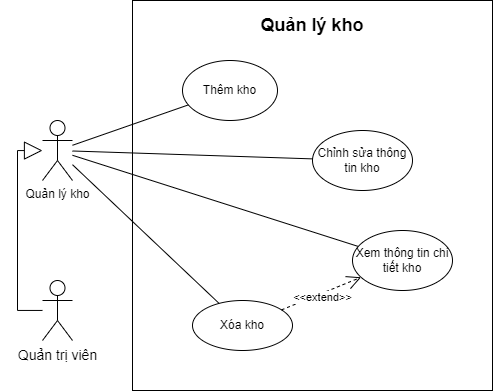
\includegraphics[width=9cm]{img/UseCase/UseCase-Quản lý kho.drawio.png}
            \newline
            \caption{Use case quản lý kho}
        \end{figure}
    
        \subsubsection{Xem thông tin chi tiết kho}
            \begin{longtable}{| p{.20\textwidth} | p{.80\textwidth} |} 
                \hline
                 \textbf{Use-case name} 
                & 
                Xem thông tin chi tiết kho.
                \\
                \hline
                \textbf{Actor} 
                & 
                Quản lý kho.
                \\
                \hline
                \textbf{Description} 
                & 
                Quản lý xem được thông tin chi tiết kho hàng mà quản lý kho muốn xem.
                \\
                \hline
                 \textbf{Preconditions} 
                &
                Quản lý kho đã đăng nhập vào hệ thống.
                \\
                \hline
                \textbf{Postconditions} 
                & 
                Quản lý xem được thông tin chi tiết kho hàng mà quản lý kho muốn xem.
                \\
                \hline
                \textbf{Trigger} 
                & 
                Quản lý kho chọn vào nút "Quản lý kho".
                \\
                \hline
                \begin{flushleft}
                 \textbf{Normal flow}
                \end{flushleft}
                & 
                1. Hệ thống hiển thị danh sách tất cả kho.
                    
                    2. Quản lý chọn kho muốn xem thông tin chi tiết và nhấp chuột vào đó.
                    
                    3. Hệ thống hiển thị thông tin chi tiết của kho mà người dùng chọn.
                    
                    4. Quản lý kho xem thông tin chi tiết của kho mà bản thân mình chọn.
                \\
                \hline
                \textbf{Alternative flow}
                & 
                Không
                %%%%%%%%%%%%%%%%
                \\
                \hline
                \textbf{Exceptions} 
                &
                Không
                %%%%%%%%%%%%%%%%%%%%
                \\
                \hline
                \caption{Đặc tả use-case \textbf{xem thông tin chi tiết kho}}
            \end{longtable}
 
        \subsubsection{Thêm kho}
            \begin{longtable}{| p{.20\textwidth} | p{.80\textwidth} |} 
                \hline
                 \textbf{Use-case name} 
                & 
                Thêm kho.
                \\
                \hline
                \textbf{Actor} 
                & 
                Quản lý kho.
                \\
                \hline
                \textbf{Description} 
                & 
                Quản lý thêm kho mới vào trong hệ thống lưu trữ.
                \\
                \hline
                 \textbf{Preconditions} 
                &
                Quản lý kho đã đăng nhập vào hệ thống.
                \\
                \hline
                \textbf{Postconditions} 
                & 
                Quản lý thêm được kho mà quản lý kho muốn.
                \\
                \hline
                \textbf{Trigger} 
                & 
                Quản lý kho chọn nút "Quản lý kho".
                \\
                \hline
                \begin{flushleft}
                 \textbf{Normal flow}
                \end{flushleft}
                & 
                1. Hệ thống hiển thị danh sách tất cả kho.
                    2. Quản lý kho chọn nút "Thêm kho".
                    
                    3. Hệ thống hiển thị thông tin kho cần điền thông tin để thêm.
                    
                    4. Người dùng nhập thông tin của kho và nhấn "Tạo".
                    
                    5. Hệ thống tiến hành kiểm tra định dạng các thông tin mà người dùng chọn và thông báo kết quả tạo kho thành công.
                    
                    6. Người dùng xem kết quả tạo kho.
                \\
                \hline
                \textbf{Alternative flow}
                & 
                Không.
                %%%%%%%%%%%%%%%%
                \\
                \hline
                \textbf{Exceptions} 
                &
                5.1. Người dùng nhập thông tin không đúng định dạng.
                    \begin{quote}
                    5.1.1. Hệ thống thông báo thông tin kho nhập vào sai định dạng, yêu cầu người dùng nhập lại.
                    
                    5.1.2. Người dùng chỉnh sửa lại các thông tin theo định dạng và chọn "Tạo".
                    
                    5.1.3.Quay lại bước 5.
                    \end{quote}
                5.2. Tạo kho thất bại.
                    \begin{quote}
                    5.2.1. Hệ thống thông báo kết quả tạo kho thất bại.
                    5.2.2. Quay lại bước 2.
                    \end{quote}
                %%%%%%%%%%%%%%%%%%%%
                \\
                \hline
                \caption{Đặc tả use-case \textbf{thêm kho}}
            \end{longtable}
    
        \subsubsection{Chỉnh sửa thông tin kho}
            \begin{longtable}{| p{.20\textwidth} | p{.80\textwidth} |} 
                \hline
                 \textbf{Use-case name} 
                & 
                Chỉnh sửa thông tin kho.
                \\
                \hline
                \textbf{Actor} 
                & 
                Quản lý kho.
                \\
                \hline
                \textbf{Description} 
                & 
                Quản lý chỉnh sửa thông tin kho.
                \\
                \hline
                 \textbf{Preconditions} 
                &
                Quản lý kho đã đăng nhập vào hệ thống.
                \\
                \hline
                \textbf{Postconditions} 
                & 
                Quản lý chỉnh sửa được thông tin của kho mà quản lý kho muốn.
                \\
                \hline
                \textbf{Trigger} 
                & 
                Quản lý chọn nút "Quản lý kho".
                \\
                \hline
                \begin{flushleft}
                 \textbf{Normal flow}
                \end{flushleft}
                & 
                1. Hệ thống hiển thị danh sách tất cả kho.
                    
                    2. Quản lý kho chọn kho muốn chỉnh sửa thông tin và nhấn nút "Chỉnh sửa".
                    
                    3. Hệ thống hiển thị thông tin kho có sẵn.
                    
                    4. Người dùng chỉnh sửa thông tin của kho và nhấn "Lưu".
                    
                    5. Hệ thống tiến hành kiểm tra định dạng các thông tin mà người dùng chọn và thông báo kết quả chỉnh sửa kho thành công.
                    
                    6. Người dùng xem kết quả chỉnh sửa kho.
                \\
                \hline
                \begin{flushleft}
                    \textbf{Alternative flow}
                \end{flushleft}
                & 
                1.1. Quản lý kho muốn chỉnh sửa sau khi xem thông tin chi tiết của kho.
                    \begin{quote}
                    1.1.1. Quản lý kho chọn nút "Chỉnh sửa" trong trang xem thông tin chi tiết kho.
                    1.1.2. Đến bước 3.
                    \end{quote}
                %%%%%%%%%%%%%%%%
                \\
                \hline
                \begin{flushleft}
                \textbf{Exceptions} 
                \end{flushleft}
                &
                5.1. Người dùng nhập thông tin không đúng định dạng.
                    \begin{quote}
                    5.1.1. Hệ thống thông báo thông tin kho nhập vào sai định dạng, yêu cầu người dùng nhập lại.
                    5.1.2. Người dùng chỉnh sửa lại các thông tin theo định dạng và chọn "Lưu".
                    5.1.3. Quay lại bước 5.
                    \end{quote}
                5.2. Hệ thống chỉnh sửa kho thất bại.
                    \begin{quote}
                    5.2.1. Hệ thống thông báo kết quả chỉnh sửa kho thất bại.
                    5.2.2. Quay lại bước 2.
                    \end{quote}
                %%%%%%%%%%%%%%%%%%%%
                \\
                \hline
                \caption{Đặc tả use-case \textbf{chỉnh sửa thông tin kho}}
            \end{longtable}
    
        \subsubsection{Xóa kho}
            \begin{longtable}{| p{.20\textwidth} | p{.80\textwidth} |} 
                \hline
                 \textbf{Use-case name} 
                & 
                Xóa kho.
                \\
                \hline
                \textbf{Actor} 
                & 
                Quản lý kho.
                \\
                \hline
                \textbf{Description} 
                & 
                Quản lý xóa kho khi thực tế không cần sử dụng nữa.
                \\
                \hline
                 \textbf{Preconditions} 
                &
                Quản lý kho đã đăng nhập vào hệ thống.
                \\
                \hline
                \textbf{Postconditions} 
                & 
                Quản lý xóa được kho mà mình muốn.
                \\
                \hline
                \textbf{Trigger} 
                & 
                Quản lý kho chọn vào nút "Quản lý kho".
                \\
                \hline
                \begin{flushleft}
                 \textbf{Normal flow}
                \end{flushleft}
                & 
                1. Hệ thống hiển thị danh sách tất cả kho.
                    
                    2.Quản lý kho chọn kho muốn xóa nhấn nút "Xóa".
                    
                    3. Hệ thống hiển thị thống báo xác nhận quản lý kho có muốn xóa kho.
                    
                    4. Quản lý chọn nút "Xác nhận".
                    
                    5. Hệ thống hiển thị kết quả xóa kho thành công.
                    
                    6. Người dùng xem kết quả xóa kho.
                \\
                \hline
                \begin{flushleft}
                    \textbf{Alternative flow}
                    
                \end{flushleft}
                & 
                1.1. Quản lý kho muốn chỉnh sửa sau khi xem thông tin chi tiết của kho.
                    \begin{quote}
                    1.1.1. Người dùng chọn nút "Xóa".
                        1.1.2 Đến bước 3.
                    \end{quote}
                %%%%%%%%%%%%%%%%
                \\
                \hline
                \begin{flushleft}
                \textbf{Exceptions} 
                \end{flushleft}
                &
                4.1. Hệ thống xóa kho thất bại.
                    \begin{quote}
                    4.1.1. Hệ thống thông báo kết quả xóa kho thất bại.
                    
                    4.1.2.Quay lại bước 1.
                    \end{quote}
                %%%%%%%%%%%%%%%%%%%%
                \\
                \hline
                \caption{Đặc tả use-case \textbf{xóa kho}}
            \end{longtable}
    


    \subsection{Quản lý hàng hóa}
        \begin{figure}[!htp]
            \centering
            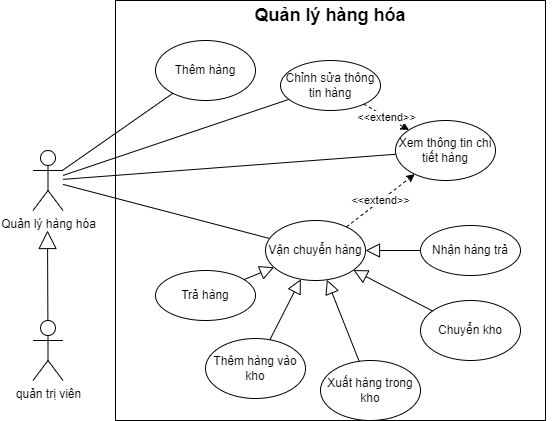
\includegraphics[width=10cm]{img/UseCase/UseCase-Quản lý hàng.drawio.png}
            \newline
            \caption{Use case quản lý hàng hóa}
        \end{figure}
        
        \subsubsection{Thêm hàng trong kho}
            \begin{longtable}{| p{.20\textwidth} | p{.80\textwidth} |} 
                \hline
                    \textbf{Use-case name} 
                & 
                    Thêm hàng trong kho
                \\
                %%%%%%%%%%%%%%%%%%
                \hline
                    \textbf{Actor} 
                & 
                    Quản lý hàng hóa
                \\
                %%%%%%%%%%%%%%%%%%
                \hline
                    \textbf{Description} 
                & 
                    Quản lý hàng hóa có thể thêm hàng vào kho
                \\
                %%%%%%%%%%%%%%%%%%
                \hline
                    \textbf{Preconditions} 
                &
                    Quản lý hàng hóa đã đăng nhập
                \\
                %%%%%%%%%%%%%%%%%%
                \hline
                    \textbf{Postconditions} 
                & 
                    Hàng được thêm
                \\
                %%%%%%%%%%%%%%%%%%
                \hline
                    \textbf{Trigger} 
                & 
                    Quản lý hàng hóa chọn "Quản lý hàng hóa"
                \\
                %%%%%%%%%%%%%%%%%%
                \hline
                \begin{flushleft}
                    \textbf{Normal flow}
                \end{flushleft}
                & 
                1. Hệ thống hiển thị danh sách hàng hóa
                    
                    2. Quản lý hàng hóa chọn "Thêm mới"
                    
                    3. Hệ thống hiển thị biểu mẫu điền thông tin
                    
                    4. Quản lý hàng hóa nhập thông tin
                    
                    5. Quản lý hàng hóa chọn "Lưu"
                    
                    6. Hệ thống cập nhật thông tin
                \\
                %%%%%%%%%%%%%%%%%%
                \hline
                \begin{flushleft}
                    \textbf{Alternative flow}
                \end{flushleft}
                &
                2.1. Hàng đã có trong kho
                    \begin{quote} 
                    2.1.1 Quản lý hàng hóa chọn vào hàng cần nhập
                        
                        2.1.2 Hệ thống hiển thị biểu mẫu thông tin quy trình
                        
                        2.1.3 Quản lý hàng hóa điền thông tin và chọn lưu
                        
                        2.1.4 Hệ thống cập nhật thông tin
                    \end{quote}
                5.1. Quản lý hàng hóa chọn hủy
                    \begin{quote} 
                    5.1.1 Quay lại bước 3
                    \end{quote}
                \\
                %%%%%%%%%%%%%%%%%%
                \hline
                    \textbf{Exceptions} 
                &
                    Không
                \\
                %%%%%%%%%%%%%%%%%%
                \hline
                \caption{Đặc tả use-case \textbf{Thêm hàng trong kho}}
            \end{longtable}

        \subsubsection{Xóa hàng trong kho}
            \begin{longtable}{| p{.20\textwidth} | p{.80\textwidth} |} 
                \hline
                    \textbf{Use-case name} 
                & 
                    Xóa hàng trong kho
                \\
                %%%%%%%%%%%%%%%%%%
                \hline
                    \textbf{Actor} 
                & 
                    Quản lý hàng hóa
                \\
                %%%%%%%%%%%%%%%%%%
                \hline
                    \textbf{Description} 
                & 
                    Quản lý hàng hóa có thể xóa hàng khỏi kho
                \\
                %%%%%%%%%%%%%%%%%%
                \hline
                    \textbf{Preconditions} 
                &
                    Quản lý hàng hóa đã đăng nhập
                \\
                %%%%%%%%%%%%%%%%%%
                \hline
                    \textbf{Postconditions} 
                & 
                    Hàng được xóa khỏi kho
                \\
                %%%%%%%%%%%%%%%%%%
                \hline
                    \textbf{Trigger} 
                & 
                    Quản lý hàng hóa chọn "Quản lý hàng hóa"
                \\
                %%%%%%%%%%%%%%%%%%
                \hline
                \begin{flushleft}
                    \textbf{Normal flow}
                \end{flushleft}
                & 
                1. Hệ thống hiển thị danh sách hàng hóa
                    
                    2. Quản lý hàng hóa tìm kiếm và chọn hàng muốn xóa
                    
                    3. Hệ thống hiển thị thông tin hàng
                    
                    4. Quản lý hàng hóa tìm kho cần xóa và chọn "Xóa"
                    
                    5. Hệ thống yêu cầu xác nhận
                    
                    6. Quản lý hàng hóa chọn "Xác nhận"
                    
                    7. Hệ thống cập nhật thông tin
                \\
                %%%%%%%%%%%%%%%%%%
                \hline
                \begin{flushleft}
                    \textbf{Alternative flow}
                \end{flushleft}
                &
                6.1. Quản lý hàng hóa chọn "Hủy"
                    \begin{quote} 
                    
                    6.1.1 Quay lại bước 3
                    \end{quote}
                \\
                %%%%%%%%%%%%%%%%%%
                \hline
                    \textbf{Exceptions} 
                &
                    Không
                \\
                %%%%%%%%%%%%%%%%%%
                \hline
                \caption{Đặc tả use-case \textbf{Xóa hàng trong kho}}
            \end{longtable}

        \subsubsection{Xem thông tin chi tiết hàng}
            \begin{longtable}{| p{.20\textwidth} | p{.80\textwidth} |} 
                \hline
                    \textbf{Use-case name} 
                & 
                    Xem thông tin chi tiết hàng
                \\
                %%%%%%%%%%%%%%%%%%
                \hline
                    \textbf{Actor} 
                & 
                    Quản lý hàng hóa
                \\
                %%%%%%%%%%%%%%%%%%
                \hline
                    \textbf{Description} 
                & 
                    Quản lý hàng hóa có thể xem thông tin đầy đủ của hàng
                \\
                %%%%%%%%%%%%%%%%%%
                \hline
                    \textbf{Preconditions} 
                &
                    Quản lý hàng hóa đã đăng nhập
                \\
                %%%%%%%%%%%%%%%%%%
                \hline
                    \textbf{Postconditions} 
                & 
                    Nhận được thông tin hàng 
                \\
                %%%%%%%%%%%%%%%%%%
                \hline
                    \textbf{Trigger} 
                & 
                    Quản lý hàng hóa chọn "Quản lý hàng hóa"
                \\
                %%%%%%%%%%%%%%%%%%
                \hline
                \begin{flushleft}
                    \textbf{Normal flow}
                \end{flushleft}
                & 
                1. Hệ thống hiển thị danh sách hàng hóa
                    
                    2. Quản lý hàng hóa tìm kiếm và chọn hàng muốn xem
                    
                    3. Hệ thống hiển thị thông tin chi tiết hàng
                \\
                %%%%%%%%%%%%%%%%%%
                \hline
                    \textbf{Alternative flow}
                &
                    Không
                \\
                %%%%%%%%%%%%%%%%%%
                \hline
                    \textbf{Exceptions} 
                &
                    Không
                \\
                %%%%%%%%%%%%%%%%%%
                \hline
                \caption{Đặc tả use-case \textbf{Xem thông tin chi tiết hàng}}
            
            \end{longtable}
        
        \subsubsection{Chỉnh sửa thông tin hàng}
            \begin{longtable}{| p{.20\textwidth} | p{.80\textwidth} |} 
                \hline
                    \textbf{Use-case name} 
                & 
                    Chỉnh sửa thông tin hàng
                \\
                %%%%%%%%%%%%%%%%%%
                \hline
                    \textbf{Actor} 
                & 
                    Quản lý hàng hóa
                \\
                %%%%%%%%%%%%%%%%%%
                \hline
                    \textbf{Description} 
                & 
                    Quản lý hàng hóa có thể thông tin đầy đủ của hàng
                \\
                %%%%%%%%%%%%%%%%%%
                \hline
                    \textbf{Preconditions} 
                &
                    Quản lý hàng hóa đã đăng nhập
                \\
                %%%%%%%%%%%%%%%%%%
                \hline
                    \textbf{Postconditions} 
                & 
                    Thông tin hàng được cập nhật
                \\
                %%%%%%%%%%%%%%%%%%
                \hline
                    \textbf{Trigger} 
                & 
                    Quản lý hàng hóa chọn "Quản lý hàng hóa"
                \\
                %%%%%%%%%%%%%%%%%%
                \hline
                \begin{flushleft}
                    \textbf{Normal flow}
                \end{flushleft}
                & 
                1. Hệ thống hiển thị danh sách hàng hóa
                    
                    2. Quản lý hàng hóa tìm kiếm và chọn hàng muốn chỉnh sửa
                    
                    3. Thông tin chi tiết hàng được hiển thị
                    
                    4. Quản lý hàng hóa chọn "Chỉnh sửa"
                    
                    5. Hệ thống hiển thị biểu mẫu thông tin hàng
                    
                    6. Quản lý hàng hóa nhập thông tin
                    
                    7. Quản lý hàng hóa chọn "Lưu"
                    
                    8. Hệ thống cập nhật thông tin
                \\
                %%%%%%%%%%%%%%%%%%
                \hline
                \begin{flushleft}
                    \textbf{Alternative flow}
                \end{flushleft}
                &
                7.1 Quản lý hàng hóa chọn "Hủy"
                    \begin{quote} 
                    7.1.1 Quay lại bước 3
                    \end{quote}
                \\
                %%%%%%%%%%%%%%%%%%
                \hline
                    \textbf{Exceptions} 
                &
                    Không
                \\
                %%%%%%%%%%%%%%%%%%
                \hline
                \caption{Đặc tả use-case \textbf{Chỉnh sửa thông tin chi tiết hàng}}
            
            \end{longtable}

        \subsubsection{Xuất hàng trong kho}
            \begin{longtable}{| p{.20\textwidth} | p{.80\textwidth} |} 
                \hline
                    \textbf{Use-case name} 
                & 
                    Xuất hàng trong kho
                \\
                %%%%%%%%%%%%%%%%%%
                \hline
                    \textbf{Actor} 
                & 
                    Quản lý hàng hóa
                \\
                %%%%%%%%%%%%%%%%%%
                \hline
                    \textbf{Description} 
                & 
                    Quản lý hàng hóa có thể xuất hảng khỏi kho
                \\
                %%%%%%%%%%%%%%%%%%
                \hline
                    \textbf{Preconditions} 
                &
                    Quản lý hàng hóa đã đăng nhập
                \\
                %%%%%%%%%%%%%%%%%%
                \hline
                    \textbf{Postconditions} 
                & 
                    Hàng được xuất khỏi kho
                \\
                %%%%%%%%%%%%%%%%%%
                \hline
                    \textbf{Trigger} 
                & 
                    Quản lý hàng hóa chọn "Quản lý hàng hóa"
                \\
                %%%%%%%%%%%%%%%%%%
                \hline
                \begin{flushleft}
                    \textbf{Normal flow}
                \end{flushleft}
                & 
                1. Hệ thống hiển thị danh sách hàng hóa
                    
                    2. Quản lý hàng hóa tìm kiếm và chọn hàng muốn xuất
                    \
                    3.Thông tin chi tiết hàng được hiển thị
                    
                    4. Quản lý hàng hóa tìm kiếm và chọn kho muốn xuất
                    
                    5. Hệ thống hiển thị biểu mẫu thông tin quy trình
                    
                    6. Quản lý hàng hóa nhập thông tin
                    
                    7. Quản lý hàng hóa chọn "Thực hiện"
                    
                    8. Hệ thống cập nhật thông tin
                \\
                %%%%%%%%%%%%%%%%%%
                \hline
                    \textbf{Alternative flow}
                &
                    Không
                \\
                %%%%%%%%%%%%%%%%%%
                \hline
                    \textbf{Exceptions} 
                &
                    Không
                \\
                %%%%%%%%%%%%%%%%%%
                \hline
                \caption{Đặc tả use-case \textbf{Xuất hàng trong kho}}
            \end{longtable}


        \subsubsection{Chuyển kho}
            \begin{longtable}{| p{.20\textwidth} | p{.80\textwidth} |} 
                \hline
                    \textbf{Use-case name} 
                & 
                    Chuyển kho
                \\
                %%%%%%%%%%%%%%%%%%
                \hline
                    \textbf{Actor} 
                & 
                    Quản lý hàng hóa
                \\
                %%%%%%%%%%%%%%%%%%
                \hline
                    \textbf{Description} 
                & 
                    Quản lý hàng hóa có thể chuyển hàng từ kho này đến kho khác
                \\
                %%%%%%%%%%%%%%%%%%
                \hline
                    \textbf{Preconditions} 
                &
                    Quản lý hàng hóa đã đăng nhập
                \\
                %%%%%%%%%%%%%%%%%%
                \hline
                    \textbf{Postconditions} 
                & 
                    Hàng chuyển đi
                \\
                %%%%%%%%%%%%%%%%%%
                \hline
                    \textbf{Trigger} 
                & 
                    Quản lý hàng hóa chọn "Quản lý hàng hóa"
                \\
                %%%%%%%%%%%%%%%%%%
                \hline
                \begin{flushleft}
                    \textbf{Normal flow}
                \end{flushleft}
                & 
                1. Hệ thống hiển thị danh sách hàng hóa
                    
                    2. Quản lý hàng hóa tìm kiếm và chọn hàng muốn xuất
                    
                    3. Thông tin chi tiết hàng được hiển thị
                    
                    4. Quản lý hàng hóa tìm kiếm và chọn kho muốn xuất
                    
                    5. Hệ thống hiển thị biểu mẫu thông tin quy trình
                    
                    6. Quản lý hàng hóa nhập thông tin
                    
                    7. Quản lý hàng hóa chọn "Thực hiện"
                    
                    8. Hệ thống cập nhật thông tin
                \\
                %%%%%%%%%%%%%%%%%%
                \hline
                    \textbf{Alternative flow}
                &
                    Không
                \\
                %%%%%%%%%%%%%%%%%%
                \hline
                    \textbf{Exceptions} 
                &
                    Không
                \\
                %%%%%%%%%%%%%%%%%%
                \hline
                \caption{Đặc tả use-case \textbf{Chuyển kho}}
            \end{longtable}

        \subsubsection{Nhận trả hàng}
            \begin{longtable}{| p{.20\textwidth} | p{.80\textwidth} |} 
                \hline
                    \textbf{Use-case name} 
                & 
                    Nhận trả hàng
                \\
                %%%%%%%%%%%%%%%%%%
                \hline
                    \textbf{Actor} 
                & 
                    Quản lý hàng hóa
                \\
                %%%%%%%%%%%%%%%%%%
                \hline
                    \textbf{Description} 
                & 
                    Quản lý hàng hóa có thể chuyển hàng từ kho này đến kho khác
                \\
                %%%%%%%%%%%%%%%%%%
                \hline
                    \textbf{Preconditions} 
                &
                    Quản lý hàng hóa đã đăng nhập
                \\
                %%%%%%%%%%%%%%%%%%
                \hline
                    \textbf{Postconditions} 
                & 
                    Hàng chuyển đi
                \\
                %%%%%%%%%%%%%%%%%%
                \hline
                    \textbf{Trigger} 
                & 
                    Quản lý hàng hóa chọn "Quản lý hàng hóa"
                \\
                %%%%%%%%%%%%%%%%%%
                \hline
                \begin{flushleft}
                    \textbf{Normal flow}
                \end{flushleft}
                & 
                1. Hệ thống hiển thị danh sách hàng hóa
                    
                    2. Quản lý hàng hóa tìm kiếm và chọn hàng muốn xuất
                    
                    3. Thông tin chi tiết hàng được hiển thị
                    
                    4. Quản lý hàng hóa tìm kiếm và chọn kho muốn xuất
                    
                    5. Hệ thống hiển thị biểu mẫu thông tin quy trình
                    
                    6. Quản lý hàng hóa nhập thông tin
                    
                    7. Quản lý hàng hóa chọn "Thực hiện"
                    
                    8. Hệ thống cập nhật thông tin
                \\
                %%%%%%%%%%%%%%%%%%
                \hline
                    \textbf{Alternative flow}
                &
                    Không
                \\
                %%%%%%%%%%%%%%%%%%
                \hline
                    \textbf{Exceptions} 
                &
                    Không
                \\
                %%%%%%%%%%%%%%%%%%
                \hline
                \caption{Đặc tả use-case \textbf{Nhận trả hàng}}
            \end{longtable}

\newpage

    \subsection{Quản lý đơn hàng}
        \begin{figure}[!htp]
            \centering
            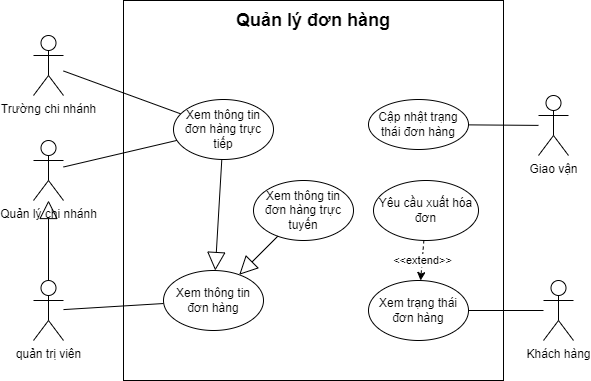
\includegraphics[width=5in]{img/UseCase/UseCase-Quản lý đơn hàng.drawio.png}
            \newline
            \caption{Use case quản lý đơn hàng}
        \end{figure}
    
    \subsubsection{Xem thông tin đơn hàng trực tiếp}
            \begin{longtable}{| p{.20\textwidth} | p{.80\textwidth} |} 
                \hline
                    \textbf{Use-case name} 
                & 
                    Xem thông tin đơn hàng trực tiếp
                \\
                %%%%%%%%%%%%%%%%%%
                \hline
                    \textbf{Actor} 
                & 
                    Quản lý chi nhánh, trưởng chi nhánh
                \\
                %%%%%%%%%%%%%%%%%%
                \hline
                    \textbf{Description} 
                & 
                    Quản lý chi nhánh, trưởng chi nhánh có thể xem thông tin các đơn hàng
                \\
                %%%%%%%%%%%%%%%%%%
                \hline
                    \textbf{Preconditions} 
                &
                    Quản lý chi nhánh, trưởng chi nhánh đã đăng nhập
                \\
                %%%%%%%%%%%%%%%%%%
                \hline
                    \textbf{Postconditions} 
                & 
                    Nhận được thông tin đơn hàng
                \\
                %%%%%%%%%%%%%%%%%%
                \hline
                    \textbf{Trigger} 
                & 
                    Quản lý chi nhánh, trưởng chi nhánh chọn "Quản lý đơn hàng"
                \\
                %%%%%%%%%%%%%%%%%%
                \hline
                \begin{flushleft}
                    \textbf{Normal flow}
                \end{flushleft}
                & 
                1. Quản lý chi nhánh, trưởng chi nhánh chọn khoảng thời gian muốn xem
                    
                    2. Hệ thống hiển thị danh sách các đơn hàng
                    
                    3. Quản lý chi nhánh, trưởng chi nhánh tìm và chọn đơn muốn xem
                    
                    4. Hệ thống hiển thị thông tin đơn hàng
                    \\
                %%%%%%%%%%%%%%%%%%
                \hline
                    \textbf{Alternative flow}
                &
                    Không
                \\
                %%%%%%%%%%%%%%%%%%
                \hline
                    \textbf{Exceptions} 
                &
                    Không
                \\
                %%%%%%%%%%%%%%%%%%
                \hline
                \caption{Đặc tả use-case \textbf{Xem thông tin đơn hàng trực tiếp}}
            \end{longtable}

    \subsubsection{Xem thông tin đơn hàng trực tuyến}
            \begin{longtable}{| p{.20\textwidth} | p{.80\textwidth} |} 
                \hline
                    \textbf{Use-case name} 
                & 
                    Xem thông tin đơn hàng trực tuyến
                \\
                %%%%%%%%%%%%%%%%%%
                \hline
                    \textbf{Actor} 
                & 
                    Quản trị viên
                \\
                %%%%%%%%%%%%%%%%%%
                \hline
                    \textbf{Description} 
                & 
                    Quản trị viên có thể xem thông tin các đơn hàng trực tuyến
                \\
                %%%%%%%%%%%%%%%%%%
                \hline
                    \textbf{Preconditions} 
                &
                    Quản trị viên đã đăng nhập
                \\
                %%%%%%%%%%%%%%%%%%
                \hline
                    \textbf{Postconditions} 
                & 
                    Nhận được thông tin đơn hàng
                \\
                %%%%%%%%%%%%%%%%%%
                \hline
                    \textbf{Trigger} 
                & 
                    Quản trị viên chọn "Đơn hàng trực tuyến" trong "Quản lý đơn hàng
                \\
                %%%%%%%%%%%%%%%%%%
                \hline
                \begin{flushleft}
                    \textbf{Normal flow}
                \end{flushleft}
                & 
                1. Quản trị viên chọn khoảng thời gian muốn xem
                    
                    2. Hệ thống hiển thị danh sách các đơn hàng
                    
                    3. Quản trị viên tìm và chọn đơn muốn xem
                    
                    4. Hệ thống hiển thị thông tin đơn hàng
                \\
                %%%%%%%%%%%%%%%%%%
                \hline
                    \textbf{Alternative flow}
                &
                    Không
                \\
                %%%%%%%%%%%%%%%%%%
                \hline
                    \textbf{Exceptions} 
                &
                    Không
                \\
                %%%%%%%%%%%%%%%%%%
                \hline
                \caption{Đặc tả use-case \textbf{Xem thông tin đơn hàng trực tuyến}}
            \end{longtable}
    
    \subsubsection{Cập nhật trạng thái đơn hàng}
            \begin{longtable}{| p{.20\textwidth} | p{.80\textwidth} |} 
    \hline
    \textbf{Use-case name} 
    & 
    Cập nhật trạng thái đơn hàng.
    \\
    \hline
    \textbf{Actor} 
    & 
    Giao vận.
    \\
    \hline
    \textbf{Description} 
    & 
        Bên giao vận gửi trạng thái cập nhật đơn hàng khi có sự thay đổi trạng thái ngoài thực tế.
    \\
    \hline
    \textbf{Preconditions} 
    &
    Bên giao vận gửi trạng thái cập nhật của đơn hàng.
    \\
    \hline
    \textbf{Postconditions} 
    & 
    Hệ thống ghi nhận trạng thái mới của đơn hàng.
    \\
    \hline
    \textbf{Trigger} 
    & 
    Không.
    \\
    \hline
    \textbf{Normal flow}
    & 
    1. Bên giao vận gửi trạng thái cập nhật của đơn hàng
        
        2. Hệ thống ghi nhận cập nhật lại trạng thái mới cho đơn hàng.
    \\
    \hline
    \textbf{Alternative flow}
    & 
    Không
    %%%%%%%%%%%%%%%%
    \\
    \hline
    \textbf{Exceptions} 
    &
    Không
    %%%%%%%%%%%%%%%%%%%%
    \\
    \hline
    \caption{Đặc tả use-case \textbf{cập nhật trạng thái đơn hàng}}
    \end{longtable}
    
    \subsubsection{Xem trạng thái đơn hàng}
    \begin{longtable}{| p{.20\textwidth} | p{.80\textwidth} |} 
    \hline
    \textbf{Use-case name} 
    & 
    Xem trạng thái đơn hàng.
    \\
    \hline
    \textbf{Actor} 
    & 
    Khách hàng.
    \\
    \hline
    \textbf{Description} 
    & 
    Khách hàng xem trạng thái hiện tại của đơn hàng.
    \\
    \hline
    \textbf{Preconditions} 
    &
    Khách hàng đã đăng nhập.
    \\
    \hline
    \textbf{Postconditions} 
    & 
    Khách hàng xem được trạng thái hiện tại của đơn hàng mà khách hàng muốn xem.
    \\
    \hline
    \textbf{Trigger} 
    & 
    Không.
    \\
    \hline
    \begin{flushleft}
    \textbf{Normal flow}
        
    \end{flushleft}
    & 
    1. Khách hàng chọn vào mục "Quản lý đơn hàng".
        
        2. Hệ thống hiển thị danh sách các đơn hàng ở tab mặc định chưa giao hàng.
        
        3. Khách hàng lựa chọn đơn hàng mà mình muốn xem thông tin và nhấn vào đơn hàng đó.
        
        4. Hệ thống hiển thị thông tin chi tiết về trạng thái đơn hàng.
        
        5. Người dùng xem kết quả trạng thái đơn hàng mà mình muốn.
    \\
    \hline
    \begin{flushleft}
        \textbf{Alternative flow}
    \end{flushleft}
    & 
    3.1. Khách hàng muốn xem các đơn hàng đã giao.
        \begin{quote}
        3.1.1. Khách hàng chọn mục "Đơn đã giao".
        
        3.1.2. Hệ thống hiển thị danh sách các đơn hàng đã giao của khách hàng.
        
        3.1.3. Quay lại bước 3.
        \end{quote}
    %%%%%%%%%%%%%%%%
    \\
    \hline
    \textbf{Exceptions} 
    &
    Không
    %%%%%%%%%%%%%%%%%%%%
    \\
    \hline
    \caption{Đặc tả use-case \textbf{xem trạng thái đơn hàng}}
    \end{longtable}
    

    \subsubsection{Yêu cầu xuất hóa đơn}
            \begin{longtable}{| p{.20\textwidth} | p{.80\textwidth} |} 
    \hline
    \textbf{Use-case name} 
    & 
    Yêu cầu xuất hóa đơn.
    \\
    \hline
    \textbf{Actor} 
    & 
    Khách hàng.
    \\
    \hline
    \textbf{Description} 
    & 
    Khách hàng yêu cầu hệ thống xuất hóa đơn cho đơn hàng online.
    \\
    \hline
    \textbf{Preconditions} 
    &
    Khách hàng đã từng mua hàng thành công trên trang bán hàng online.
    \\
    \hline
    \textbf{Postconditions} 
    & 
    Hệ thống gửi khách hàng hóa đơn của đơn hàng tương ứng.
    \\
    \hline
    \textbf{Trigger} 
    & 
    Không.
    \\
    \hline
    \begin{flushleft}
        \textbf{Normal flow}
    \end{flushleft}
    & 
    1. Khách hàng chọn vào mục "Quản lý đơn hàng".
        
        2. Hệ thống hiển thị danh sách các đơn hàng ở tab mặc định chưa giao hàng.
        
        3. Khách hàng chọn mục "Đơn đã giao".
        
        4. Hệ thống hiển thị danh sách các đơn hàng đã giao của khách hàng.
        
        5. Khách hàng lựa chọn đơn hàng mà mình muốn xem thông tin và nhấn vào đơn hàng đó sau đó chọn "Yêu cầu xuất hóa đơn".
        
        6. Hệ thống thông báo kết quả và trả về tệp hóa đơn cho khách hàng.
        
        7. Người dùng xem kết quả trong tệp hóa đơn.
    \\
    \hline
    \textbf{Alternative flow}
    & 
    Không
    %%%%%%%%%%%%%%%%
    \\
    \hline
    \begin{flushleft}
        \textbf{Exceptions} 
    \end{flushleft}
    &
    3.1. Hệ thống tạo hóa đơn thất bại.
        \begin{quote}
        3.1.1. Quay lại bước 3.
        \end{quote}
    %%%%%%%%%%%%%%%%%%%%
    \\
    \hline
    \caption{Đặc tả use-case \textbf{yêu cầu xuất hóa đơn}}
    \end{longtable}
    
            
            